\documentclass[10pt,letterpaper]{article}

\usepackage[top=0.85in,left=2.75in,footskip=0.75in]{geometry}
\usepackage{changepage}

% OLIVER: The next line should be uncommented, but generates an error at present
%\usepackage[utf8]{inputenc}

\usepackage{textcomp}
\usepackage{marvosym}
\usepackage{fixltx2e}
\usepackage{cite}
\usepackage{nameref}
\usepackage[right]{lineno}
\usepackage{rotating}
\usepackage[numbers]{natbib}

\usepackage[T1]{fontenc}
\usepackage{lmodern}
\usepackage{amssymb,amsmath}
\usepackage{ifxetex,ifluatex}

% OLIVER: The next two lines should be uncommented, but generate an error at present
%\usepackage{microtype}
%\DisableLigatures[f]{encoding = *, family = * }

% OLIVER: Remove comment for double spacing
\usepackage{setspace} 
\doublespacing

\raggedright
\setlength{\parindent}{0.5cm}
\textwidth 5.25in 
\textheight 8.75in

\usepackage[aboveskip=1pt,labelfont=bf,labelsep=period,justification=raggedright,singlelinecheck=off]{caption}

\bibliographystyle{plos2015}

\makeatletter
\renewcommand{\@biblabel}[1]{\quad#1.}
\makeatother

\date{}

\setlength{\bibsep}{0.0pt}

% Header and Footer with logo
\usepackage{lastpage,fancyhdr,graphicx}
\usepackage{epstopdf}
\pagestyle{myheadings}
\pagestyle{fancy}
\fancyhf{}
\lhead{\includegraphics[width=2.0in]{PLOS-submission.pdf}}
\rfoot{\thepage/\pageref{LastPage}}
\renewcommand{\footrule}{\hrule height 2pt \vspace{2mm}}
\fancyheadoffset[L]{2.25in}
\fancyfootoffset[L]{2.25in}
\lfoot{\sf PLOS}

%% Include all macros below

\newcommand{\lorem}{{\bf LOREM}}
\newcommand{\ipsum}{{\bf IPSUM}}
\renewcommand{\includegraphics}[2][]{}

% OJM - pandoc issue
\def\tightlist{}

%% END MACROS SECTION



% use upquote if available, for straight quotes in verbatim environments
\IfFileExists{upquote.sty}{\usepackage{upquote}}{}
\ifnum 0\ifxetex 1\fi\ifluatex 1\fi=0 % if pdftex
  \usepackage[utf8]{inputenc}
\else % if luatex or xelatex
  \ifxetex
    \usepackage{mathspec}
    \usepackage{xltxtra,xunicode}
  \else
    \usepackage{fontspec}
  \fi
  \defaultfontfeatures{Mapping=tex-text,Scale=MatchLowercase}
  \newcommand{\euro}{€}
\fi
% use microtype if available
\IfFileExists{microtype.sty}{\usepackage{microtype}}{}

\usepackage{graphicx}
% Redefine \includegraphics so that, unless explicit options are
% given, the image width will not exceed the width of the page.
% Images get their normal width if they fit onto the page, but
% are scaled down if they would overflow the margins.
\makeatletter
\def\ScaleIfNeeded{%
  \ifdim\Gin@nat@width>\linewidth
    \linewidth
  \else
    \Gin@nat@width
  \fi
}
\makeatother
\let\Oldincludegraphics\includegraphics
{%
 \catcode`\@=11\relax%
 \gdef\includegraphics{\@ifnextchar[{\Oldincludegraphics}{\Oldincludegraphics[width=\ScaleIfNeeded]}}%
}%
\ifxetex
  \usepackage[setpagesize=false, % page size defined by xetex
              unicode=false, % unicode breaks when used with xetex
              xetex]{hyperref}
\else
  \usepackage[unicode=true]{hyperref}
\fi
\hypersetup{breaklinks=true,
            bookmarks=true,
            pdfauthor={O.J. Maclaren\^{}1*, A. Parker\^{}2, C. Pin\^{}2, S.R. Carding\^{}\{2,3\}, A.J.M. Watson\^{}\{2,3\}, A.G. Fletcher\^{}\{4,5\}, H.M. Byrne\^{}6 and P.K. Maini\^{}6},
            pdftitle={A hierarchical Bayesian model for understanding the spatiotemporal dynamics of the intestinal epithelium},
            colorlinks=true,
            citecolor=blue,
            urlcolor=blue,
            linkcolor=magenta,
            pdfborder={0 0 0}}
\urlstyle{same}  % don't use monospace font for urls
\setlength{\parindent}{0pt}
\setlength{\parskip}{6pt plus 2pt minus 1pt}
\setlength{\emergencystretch}{3em}  % prevent overfull lines
\setcounter{secnumdepth}{0}
\usepackage{unicode-math}
\usepackage{fncylab}
\usepackage[right]{lineno}
\usepackage{tikz-cd}
\usepackage{textcomp}

\title{A hierarchical Bayesian model for understanding the spatiotemporal
dynamics of the intestinal epithelium}
\author{O.J. Maclaren\(^1\)*, A. Parker\(^2\), C. Pin\(^2\), S.R.
Carding\(^{2,3}\), A.J.M. Watson\(^{2,3}\), A.G. Fletcher\(^{4,5}\),
H.M. Byrne\(^6\) and P.K. Maini\(^6\)}
\date{}

\begin{document}
\vspace*{0.35in}
\begin{flushleft}
{\Large
\textbf\newline{A hierarchical Bayesian model for understanding the spatiotemporal
dynamics of the intestinal epithelium}
}
\newline
\\
O.J. Maclaren\(^1\)*, A. Parker\(^2\), C. Pin\(^2\), S.R.
Carding\(^{2,3}\), A.J.M. Watson\(^{2,3}\), A.G. Fletcher\(^{4,5}\),
H.M. Byrne\(^6\) and P.K. Maini\(^6\)
\end{flushleft}


\textbf{1 Department of Engineering Science, University of Auckland,
Auckland, New Zealand}\\
\textbf{2 Gut Health and Food Safety Research Programme, Institute of
Food Research, Norwich, United Kingdom}\\
\textbf{3 Norwich Medical School, University of East Anglia, Norwich,
United Kingdom}\\
\textbf{4 School of Mathematics and Statistics, University of Sheffield,
Sheffield, United Kingdom}\\
\textbf{5 Bateson Centre, University of Sheffield, Sheffield, United
Kingdom}\\
\textbf{6 Wolfson Centre for Mathematical Biology, Mathematical
Institute, University of Oxford, Oxford, United Kingdom}\\
*\textbf{oliver.maclaren@auckland.ac.nz}

\section{Abstract}\label{abstract}

Our work addresses two key challenges, one biological and one
methodological. First, we aim to understand how proliferation and cell
migration rates in the intestinal epithelium are related under healthy,
damaged (Ara-C treated) and recovering conditions, and how these
relations can be used to identify mechanisms of repair and regeneration.
We analyse new data, presented in more detail in a companion paper, in
which BrdU/IdU cell-labelling experiments were performed under these
respective conditions. Second, in considering how to more rigorously
process these data and interpret them using mathematical models, we use
a probabilistic, hierarchical approach. This provides a best-practice
approach for systematically modelling and understanding the
uncertainties that can otherwise undermine the generation of reliable
conclusions - uncertainties in experimental measurement and treatment,
difficult-to-compare mathematical models of underlying mechanisms, and
unknown or unobserved parameters. Both spatially discrete and continuous
mechanistic models are considered and related via hierarchical
conditional probability assumptions. We perform model checks on both
in-sample and out-of-sample datasets and use them to show how to test
possible model improvements and assess the robustness of our
conclusions. We conclude, for the present set of experiments, that a
primarily proliferation-driven model suffices to predict labelled cell
dynamics over most time-scales.

\section{Author Summary}\label{author-summary}

The intestinal epithelium is an important model system for studying the
dynamics and regulation of multicellular populations. It is
characterised by rapid rates of self-renewal and repair; dysregulation
of these processes is thought to explain, in part, why many tumours form
in the intestinal and similar epithelial tissues. These features have
led to a large amount of work on estimating cell kinetic parameters in
the intestine. There remain, however, large gaps between the raw data
collected, the interpretation of these experimental data, and
mechanistic models that describe the underlying processes. Hierarchical
statistical modelling provides a natural method with which to bridge
these gaps, but has, to date, been underutilised in the study of
intestinal tissue self-renewal. As we illustrate, this approach makes
essential use of the distinction between `measurement', `process' and
`parameter' models, giving an explicit framework for combining
experimental data and mechanistic modelling in the presence of multiple
sources of uncertainty. We apply this approach to analyse experiments on
healthy, damaged and recovering intestinal tissue, finding that observed
data can be explained by a model in which cell movement is driven
primarily by proliferation.

\linenumbers

\section{Introduction}\label{introduction}

\subsection{Motivation}\label{motivation}

The intestinal epithelium provides crucial barrier, transport and
homeostatic functions. These requirements lead it to undergo constant
repair and regeneration, and dysfunctions can result in pathologies such
as tumorigenesis {[}1--7{]}. Much work has been carried out on
estimating the rate parameters in the intestine and other epithelia
{[}1, 8--10{]}. However, attempts to interpret these experimental data
using mechanistic modelling remain inconclusive {[}11--14{]}, due to the
lack of consistent and reproducible approaches for comparing models
representing conjectured biological mechanisms, both to each other and
to experimental data.

This challenge goes in both directions: using experimental data (taken
to be `true') to parameterise and test mathematical or computational
formalisations of mechanistic theories, and using these models (taken to
be `true') to predict, interpret and question experimental results. Both
experimental measurements and mathematical models are subject to
uncertainty, and we hence need systematic ways of quantifying these
uncertainties and attributing them to the appropriate sources.
Furthermore, establishing a common approach for analysing experimental
results, formulating mechanistic models and generating new predictions
has many potential advantages for enabling interdisciplinary teams to
communicate in a common language so that they may efficiently discover
and follow promising directions as and when they arise.

\subsection{Approach}\label{approach}

We address the above issues by developing a hierarchical Bayesian model
for combining measurements, models and inference procedures, and
applying it to a set of experiments targeting mechanisms of repair and
regeneration in the intestinal epithelium.

While progress is now being made in tackling this challenge in other
areas of biology (see, for example, {[}15--17{]}), to our knowledge the
problem of intestinal epithelial dynamics has not yet been investigated
using such an approach.

The experiments under investigation were performed by ourselves and are
presented in more detail in {[}18{]}. The aim of these experiments was
to determine how proliferation rates, tissue growth and cellular
migration rates are related under healthy, damaged (Ara-C treated) and
recovering conditions, and how these relations can be used to identify
mechanisms of repair and regeneration.

A notable feature of the Bayesian approach to probabilistic modelling is
that all sources of uncertainty are represented via probability
distributions {[}19--21{]}. Adopting this perspective, we consider both
observations and parameters to be random variables. Within a modelling
context, uncertainty may be associated with (at least): parameters
within a mechanistic model of a biological or physical process, the
mechanistic model of the process itself and the measurements of the
underlying process. This leads, initially, to the postulation of a full
joint probability distribution for observable, unobservable/unobserved
variables, parameters and data.

Another key feature of the Bayesian perspective is that it provides a
natural way of decomposing such full joint models in a
\emph{hierarchical} manner, e.g.~by separating out processes occurring
on different scales and at different analysis stages. A given set of
hierarchical assumptions corresponds to assuming a factorisation of the
full joint distribution mentioned above, and gives a more interpretable
and tractable starting point.

Our factorisation follows that described in {[}21--24{]}. This
comprises: a `measurement model', which defines the observable (sample)
features to be considered reproducible and the precision with which they
are reproducible (the measurement scale); an underlying `process' model,
which captures the key mechanistic hypotheses of spatiotemporal
evolution, and a prior parameter model which defines a broad class of
\emph{a priori} acceptable parameter values.

In order to illustrate some of the modelling benefits of the
hierarchical approach, we show how both discrete and continuous process
models can be derived and related using the hierarchical perspective. We
discuss the relationship between the conditional/hierarchical modelling
and causal modelling literatures (see {[}25--27{]} for reviews) and
illustrate the distinct roles of (Bayesian) predictive distributions
vs.~parameter distributions for model checking and the assessment of
evidence, respectively {[}20, 28--31{]}.

\subsection{Conclusions}\label{conclusions}

Our hierarchical Bayesian model incorporates measurement, process and
parameter models and facilitates separate checking of these components.
This checking indicates, in the present application to the
spatiotemporal dynamics of the intestinal epithelium, that much of the
observed measurement variability can be adequately captured by a simple
measurement model. Similarly we find that a relatively simple process
model can account for the main spatiotemporal dynamics of interest;
however, model checking also identifies a minor misfit in the process
model appearing over long time-scales. This motivates possible model
improvements: we consider the inclusion of additional finite-cell-size
effects in the process model, derived from a discrete process model and
a subsequent continuum approximation formulated in terms of conditional
probability. This only gives a slightly better qualitative fit to
experimental data, however. We instead find that the dominant sources of
the long-time misfits are probably due to some other factors - most
likely relatively slow, time-varying proliferation rates (e.g.~due to
circadian rhythms). In summary, a primarily proliferation-driven model
appears adequate for predictions over moderate time-scales.

\section{Materials and methods I: Experimental treatments and data
processing}\label{materials-and-methods-i-experimental-treatments-and-data-processing}

\subsection{Homeostasis mouse model}\label{homeostasis-mouse-model}

To estimate intestinal epithelial cell proliferation and migration rates
under normal, homeostatic conditions in healthy mice, we used standard
methods of proliferative cell labelling and tracing {[}1, 8--10,
32--34{]} (see also {[}18{]} for full details). Actively proliferating
cells in the intestinal crypts were labelled by single injection of the
thymine analogue 5-bromo-2-deoxyuridine (BrdU) and labelled cells
detected by immunostaining of intestinal sections collected from
different individuals over time. Migration of labelled cells traced from
the base of crypts to villus tips was monitored over the course of 96
hours (5760 min). At least 30 such strips were analysed per mouse. The
figures presented in {[}18{]} reveal that these strips were independent
and obtained from one-cell thick sections. All strips in which the base
of the crypt and the tip of the villus were clearly observed were
considered. All sides of the crypt that were visible and connected to
entire villi were analysed. A typical image from those analysed in
{[}18{]} is shown in Supplementary Figure 4.

\subsection{Blocked-proliferation mouse
model}\label{blocked-proliferation-mouse-model}

To assess the effects of proliferation inhibition on crypt/villus
migration, migrating and proliferating epithelial cells were monitored
by double labelling with two thymine analogues (BrdU and IdU),
administered sequentially a number of hours apart and subsequently
distinguished by specific immunostaining in longitudinal sections of
small intestine. Following initial IdU labelling of proliferating cells
at t= -17h (-1020 min, relative to Ara-C treatment), mice were then
treated with cytosine arabinoside (Ara-C) at 250 mg/kg body weight, a
dose reported to inhibit proliferation without causing major crypt cell
atrophy (see {[}18{]} and references therein for details). Tissues were
collected over 24 hours, with BrdU administered one hour prior to
collection to check for residual proliferation. Successful inhibition of
proliferation following treatment with Ara-C was confirmed by an absence
of BrdU (S-phase) and phospho-Histone H3 (pH3) staining (M-phase) in
longitudinal sections of small intestine (again, see {[}18{]} for full
details).

\subsection{Recovering-proliferation mouse
model}\label{recovering-proliferation-mouse-model}

The above Ara-C treatment effect was observed to last for at least 10h
(600 min). Cell proliferation returned to near normal levels in samples
obtained 18h (1080 min) post-Ara-C treatment. We hence considered
samples collected at least 10h post-Ara-C treatment as corresponding to
`recovering-proliferation' conditions.

\subsection{Data processing: reference grid and key observable
features}\label{data-processing-reference-grid-and-key-observable-features}

To relate experimental measurements to the mechanistic models discussed
below we specified a reference grid and defined the key features of the
data relative to this grid. These key features established an ideal
`underlying population' from which samples were considered to be drawn.
This also allowed us to construct our hierarchical model in a
(data-to-parameter) manner, starting from a measurement model.

\begin{figure}
\centering
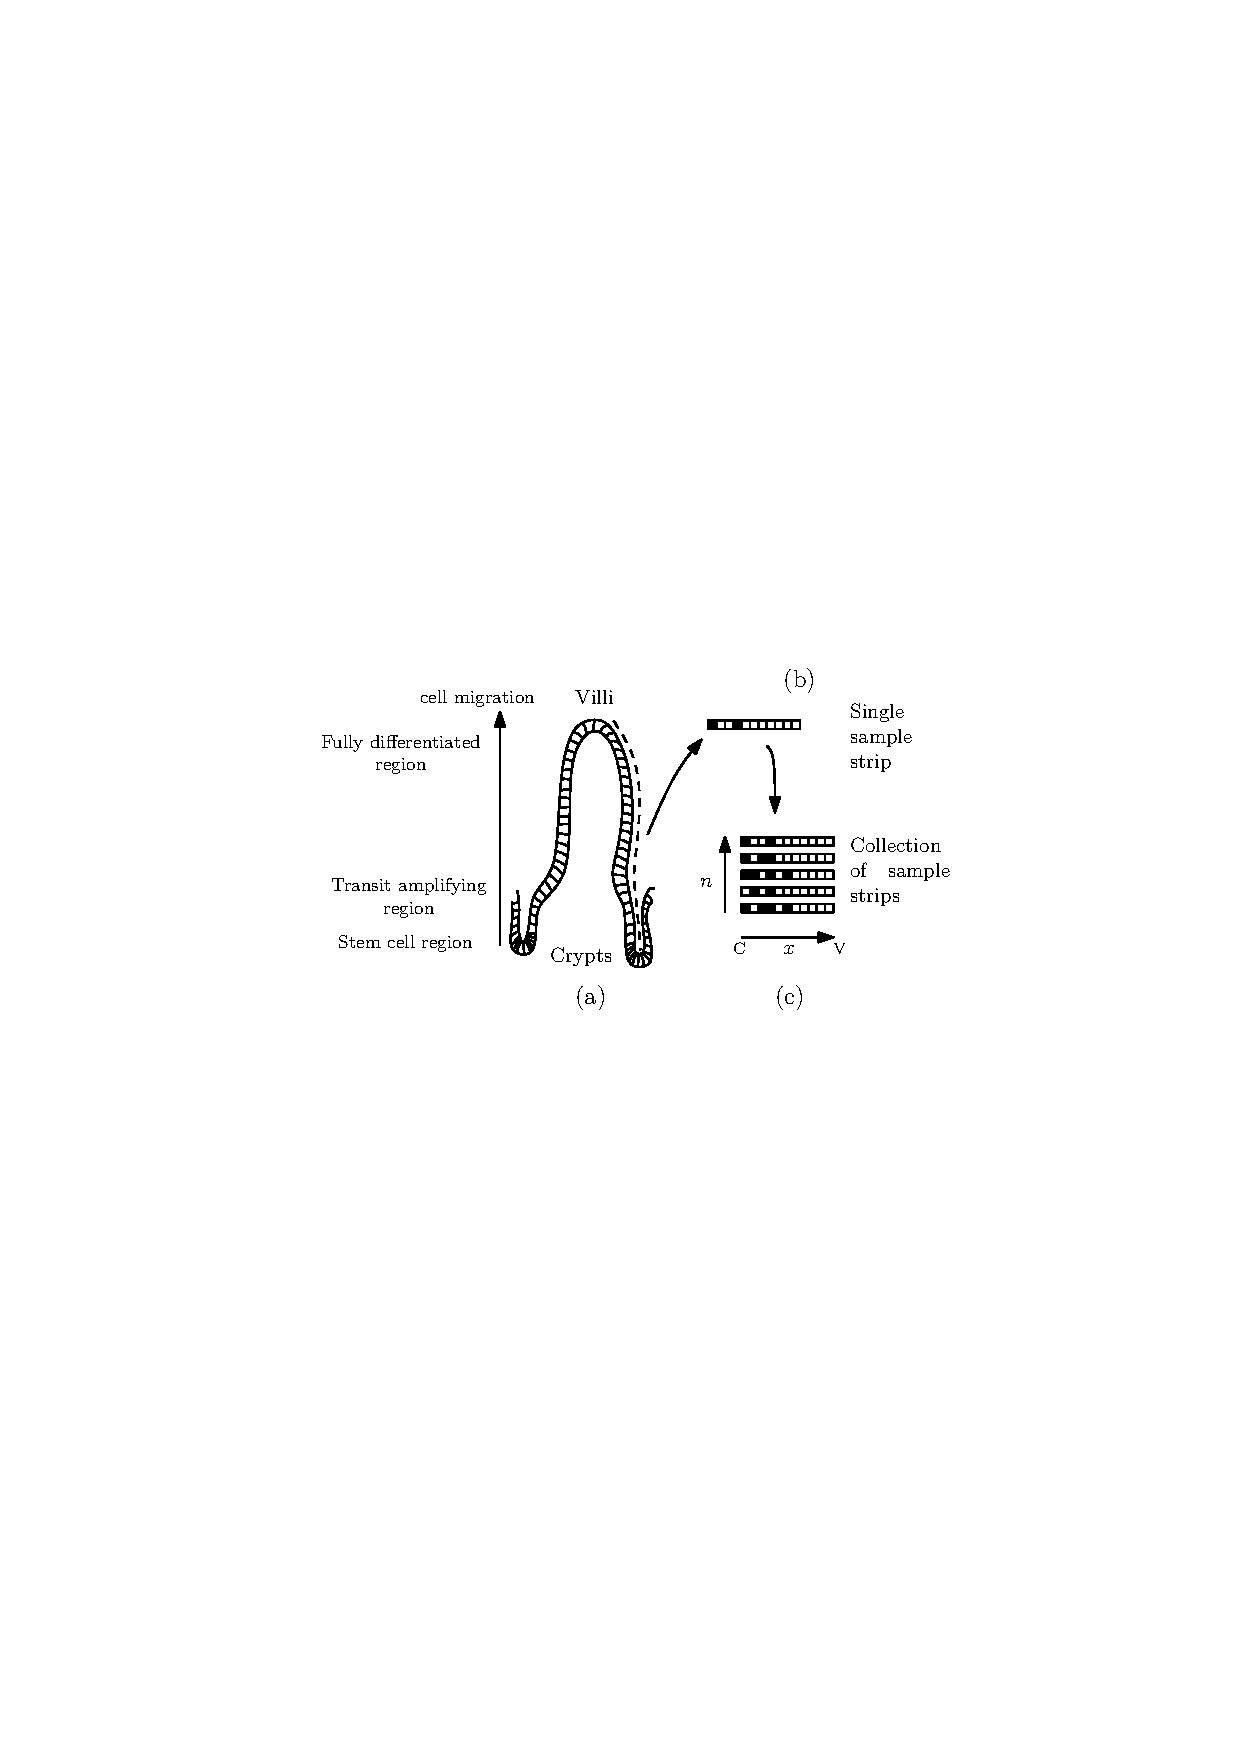
\includegraphics[draft]{../figures/figures_to_include/Fig1}
\caption{The (a) intestinal epithelium, (b) individual measurements as
strips of cells and (c) collection of strips, where `C' and `V'
indicated `crypt' and `villus'
respectively.\label{fig:intestine-measurement}}
\end{figure}

With reference to Fig \ref{fig:intestine-measurement}, we viewed the
data as a collection of one-dimensional `strips' of cells. The strips
extended from the base of the crypt to the tip of the villus, along the
so-called `crypt-villus' axis. This corresponds to how strips were
collected experimentally, but does not account for possible biases due
to `angled' sampling {[}35, 36{]}. Each measurement was given a spatial
cell location index \(i\) and a time label \(t\). The location index was
measured in numbers of cells along the crypt-villus axis, starting from
the crypt base, and hence defined a discrete one-dimensional grid.

When notationally convenient, the labels \(i\) and \(t\) were combined
in a two-dimensional grid of space-time points via the single index
parameter \(s := (i,t)\). A `typical' reference crypt-villus unit was
characterised by the two vectors \((\mathbf{L},\mathbf{n})\), where
\(\mathbf{L}\) is the vector of underlying labelled fractions
(i.e.~occupancy probabilities) at each grid point and \(\mathbf{n}\) is
the vector of number of samples at each grid point. This defines a
useful reduction of the system from two spatial dimensions to one.

We assumed that each strip was independent of the others as, in general,
strips were taken from different crypt-villus units and/or animals after
`identical preparation'. Thus we did not ever directly possess, for
example, measurements of a particular crypt with dimensions given in
terms of a certain number of strips. We note, however, that the dynamics
of strips in a given crypt may be affected by those in the same crypt.
We did not consider this additional complexity in the present work, and
so this complication should be kept in mind when interpreting the
results.

\section{Materials and methods II: Mathematical
model}\label{materials-and-methods-ii-mathematical-model}

Our hierarchical probability model was constructed on the basis of
conditional probability assumptions. These allowed us to factor out a
measurement model, a mechanistic model and a parameter model.

\subsection{Overall hierarchical
structure}\label{overall-hierarchical-structure}

Our model structure consisted of a full joint distribution, conditioned
on a given experimental treatment \(E\) and known sample size vector
\(\mathbf{n}\), decomposed according to

\begin{equation}p(\mathbf{y},\mathbf{L},\mathbf{k}|\mathbf{n},E) = p(\mathbf{y}|\mathbf{L},\mathbf{n})p(\mathbf{L}|\mathbf{k})p(\mathbf{k}|E),\label{eq:decomp}\end{equation}

where \(\mathbf{k}\) are the cellular proliferation rates (these are
discussed below). This hierarchical factorisation corresponds to the
assumption of conditional independence between the various levels, i.e.
\(p(\mathbf{y}|\mathbf{L},\mathbf{k},\mathbf{n},E) = p(\mathbf{y}|\mathbf{L},\mathbf{n})\),
\(p(\mathbf{L}|\mathbf{k},\mathbf{n},E) = p(\mathbf{L}|\mathbf{k})\) and
\(p(\mathbf{k}|\mathbf{n},E) = p(\mathbf{k}|E)\). The first term,
\(p(\mathbf{y}|\mathbf{L},\mathbf{n})\) is the \emph{measurement model};
the second term \(p(\mathbf{L}|\mathbf{k})\) is the underlying
\emph{process model}, and the last term \(p(\mathbf{k}|E)\) is a
\emph{prior parameter model}. These are discussed in turn below.

Notably, a `causal' (structural invariance) assumption {[}25--27,
37--42{]} is made by assuming that the experimental treatment condition
affects the process parameters \(\mathbf{k}\) but not the structure of
the measurement or process models. In particular, while the experimental
treatment ultimately affects \(\mathbf{y}\), in our model it does so
\emph{via} its effect on \(\mathbf{k}\) and \(\mathbf{k}\)'s subsequent
effect on \(\mathbf{L}\). This leads to the conditional independence
structure mentioned. In terms of so-called directed acyclic graphs
(DAGs), used in the causal modelling literature referenced above, we
assumed

\begin{equation}
\begin{tikzcd}
E \arrow[r] & \mathbf{k} \arrow[r] & \mathbf{L} \arrow[r] & \mathbf{y}. 
\end{tikzcd}
\label{eq:dag}\end{equation}

Another way of stating this is that knowledge of \(\mathbf{L}\) (and
\(\mathbf{n}\)) is sufficient to determine \(\mathbf{y}\) regardless of
how \(\mathbf{L}\) was brought about, but that to know \(\mathbf{L}\) we
(ultimately) have to know which experiment was carried out. Note that in
general we suppressed, in our notation, the explicit conditioning on
sample size \(\mathbf{n}\), since it was taken to be fixed and known, as
well as the conditioning on \(E\) (keeping in mind that it was assumed
to only affect \(\mathbf{k}\)).

The assumptions underlying the above factorisation could be checked to
some extent. This relied on a distinction between working `within' the
model - e.g.~parameter estimation assuming the model and factorisation
is valid - and working `outside' the model, e.g.~checking the validity
of the model structural assumptions themselves {[}20, 30, 31{]}. This
distinction is made in the Results section.

Implicit in the model derivations, discussed below, we used a
\emph{deterministic expression of conservation of probability} for the
process model, as is typical for such equations {[}43{]}. It sufficed
for the presentation here to simply replace all functional dependencies
on the process variable above with a dependence on the process
parameters {[}21{]}.

We provide further discussion of our approach to interpretation of
statistical evidence in the Supplementary Information.

\subsection{Bayesian framework for predictions and incorporating
information from
observations}\label{bayesian-framework-for-predictions-and-incorporating-information-from-observations}

The overall model of the previous section defined our initial
`generative' probabilistic model, prior to explicitly incorporating
information from our experimental data. This enabled samples to be drawn
from both prior predictive and prior parameter models, in the usual way
(see e.g. {[}20, 44{]} and the Computational methods section below). In
particular, the prior predictive distribution was used in its usual form

\begin{equation}\mathbf{y} \sim p(\mathbf{y}) = \int p(\mathbf{y}|f(\mathbf{k}))p(\mathbf{k})d\mathbf{k}\label{eq:prior-predictive}\end{equation}

which incorporates the aforementioned deterministic link between a given
sample of process parameters and the output process variable,
\(\mathbf{L}=f(\mathbf{k})\). Note that here \(\sim\) denotes
`distributed as', or more relevantly, `samples drawn according to'.

To incorporate new data \(\mathbf{y_0}\) we updated the parameters of
the model, hence passing to a `posterior predictive' model {[}20{]}

\begin{equation}\mathbf{y} | \mathbf{y_0} \sim p(\mathbf{y}|\mathbf{y_0}) = \int p(\mathbf{y}|f(\mathbf{k}))p(\mathbf{k}|\mathbf{y_0})d\mathbf{k}\label{eq:posterior-predictive}\end{equation}

where we used the conditional probability closure assumption
\(p(\mathbf{y}|f(\mathbf{k}),\mathbf{y_0}) = p(\mathbf{y}|f(\mathbf{k}))\).
This closure assumption can be interpreted as maintaining our same
mechanistic model despite new observations.

\subsection{Measurement model}\label{measurement-model}

The measurement model \(p(\mathbf{y}|\mathbf{L},\mathbf{n})\) component
was taken to be a binomial distribution \(\mathcal{B}\) of the form

\begin{align}p(\mathbf{y}|\mathbf{L},\mathbf{n}) = \underset{s=0}{\overset{S-1}{\Pi}}\mathcal{B}(n_s,L_s).\end{align}

This related our `raw' observable \(\mathbf{y}\), the vector of counts
of labelled cells at each grid point, to `ideal characteristics' of
comparison \((\mathbf{L},\mathbf{n})\). We took the measurement
component to be independent of the experimental treatment \(E\),
i.e.~treatment was assumed to affect the underlying \emph{process
parameters} only (see `Overall hierarchical structure' section). The
measurement component \(p(\mathbf{y}|\mathbf{L},\mathbf{n})\) then
defined a likelihood function \(\mathcal{L}\) for this measurement
model,

\begin{equation}\mathcal{L}(\mathbf{L};\mathbf{y},\mathbf{n}) = \underset{s=0}{\overset{S-1}{\Pi}}
L_s^{y_s}(1-L_s)^{n_s-y_s} \propto p(\mathbf{y}|\mathbf{L},\mathbf{n}) = \underset{s=0}{\overset{S-1}{\Pi}}\mathcal{B}(n_s,L_s).\label{eq:likel-binom}\end{equation}

When interpreting model misfit based on residuals, we applied the usual
normal approximation to the binomial distribution. In that case,
denoting the set of all measured labelled fractions through the (useful,
but slightly non-standard) notation
\(\mathbf{y}/\mathbf{n} := (y_1/n_1,...,y_S/n_S)\), we have

\begin{equation}\mathcal{L}(\mathbf{L};\mathbf{n},\frac{\mathbf{y}}{\mathbf{n}}) = p(\frac{\mathbf{y}}{\mathbf{n}}|\mathbf{L},\mathbf{n}) =
\underset{s=0}{\overset{S-1}{\Pi}} \frac{1}{\sigma_s
\sqrt{2\pi}}\exp{(-\frac{(\frac{y_s}{n_s}-L_s)^2}{2\sigma_s^2})}\label{eq:likel-norma}\end{equation}

where the standard deviations are given by
\(\sigma_s = \sqrt{\frac{L_s(1-L_s)}{n_s}}\).

\subsection{Process models}\label{process-models}

We developed our process model at different levels of resolution. First,
we considered a spatially discrete probabilistic model at the level of
our measurement grid defined above. Second, we considered two spatially
continuous approximations: one model excluding explicit cell-scale
effects and one including them.

\subsubsection{Spatially discrete process
model}\label{spatially-discrete-process-model}

Our basic `process' model described the evolution of the occupancy
probabilities (population labelled fractions) at the scale of the
measurement grid. This was derived as follows. With reference to Fig
\ref{fig:intestine-measurement}, we considered a collection of
one-dimensional `strips' of cells. We used \(l_i \in \{0,1\}\) as an
indicator variable denoting the occupancy status of site \(i\) of a
given strip. The full state of this strip was given by the vector
\(\mathbf{l} = (l_0,l_1,...l_{S-1})\). We then sought a description of
the probabilistic dynamics in terms of a discrete-time Markov chain for
the probability distribution of the full state \(p(\mathbf{l},t)\)
following standard arguments {[}43, 45{]}.

We began from an explicit joint distribution for the full state and then
reduced it to a description in terms of the set of `single-site'
probability distributions \(p(l_i,t)\) for each site \(i\). This
derivation was aided by adopting an explicit notation: the probabilities
of occupancy and vacancy at site \(i\) at time \(t\) were denoted by
\(p(l_i(t)=1)\) and \(p(l_i(t)=0)\) respectively. Since
\(p(l_i(t)=1)+ p(l_i(t)=0) = 1\) we only needed to consider the
probability of occupancy to fully characterise the distribution
\(p(l_i(t))\).

The equation of evolution for this probability was derived by
considering conservation of probability in terms of probability fluxes
in and out, giving, to first order in \(\Delta t\),

\begin{align}p(l_i(t+\Delta t)=1) &- p(l_i(t)=1) = \nonumber \\ &\Delta t\sum_{j=0}^{i-1}k_j\left[p(l_{i-1}(t)=1,l_{i}(t)=0)-p(l_{i-1}(t)=0,l_{i}(t)=1)\right]. \end{align}

The first term on the right represents a net `influx of occupancy
probability' due to a single division event at site \(j < i\), each
division event having a probability \(k_j\Delta t\). This flux means the
value of the state variable \(l_i(t) = 0\) could be replaced, at the
next time step, by the value of \(l_{i-1}(t) = 1\). Similarly the second
term represents a net `outflux of occupancy probability' due to a
division event at site \(j < i\). Partitioning on the events
\(l_{i-1}(t)=0\) and \(l_i(t)\), we obtain

\begin{equation}p(l_i(t+\Delta t)=1) - p(l_i(t)=1) = \Delta t\sum_{j=0}^{i-1}k_j\left[p(l_{i-1}(t)=1)-p(l_i(t)=1)\right]. \label{eq:label-master-discrete-cons}\end{equation}

\subsubsection{Underlying continuous model - zeroth-order
approximation}\label{underlying-continuous-model---zeroth-order-approximation}

To aid model interpretation and model cross comparisons we derived a
continuous approximation to the occupancy probability, \(L(x,t)\). This
gave a further idealisation of the `underlying population' from which we
envisaged the strips were sampled. This smoothness assumption, while not
strictly necessary, meant some model properties could be interpreted in
terms of local derivatives; it also reduced arbitrary dependence on
discrete grid features, aiding future comparisons with off-lattice
and/or continuum models {[}44{]}.

As detailed in the Supplementary Information, \(L(x,t)\) satisfies the
equation

\begin{equation}\frac{\partial L(x,t)}{\partial t} + v(x)\frac{\partial L(x,t)}{\partial x} = 0\label{eq:model-pde}\end{equation}

with

\begin{equation}v(x) = \int_0^{x} k(x') dx',\label{eq:model-veloc}\end{equation}

where \(k(x)\) denotes the (net) proliferation rate.

\subsubsection{Underlying continuous model - higher-order spatial
effects}\label{underlying-continuous-model---higher-order-spatial-effects}

Our `zeroth-order' continuous approximation above was obtained by
neglecting all higher-order terms in \(\Delta x\). We anticipate that a
more accurate continuum approximation may be obtained by retaining
higher-order spatial derivatives and hence finite-cell-size effects.
This gives rise to a Fokker-Planck equation containing a diffusion term
{[}43{]}:

\begin{equation}\frac{\partial L(x,t)}{\partial t} + v(x)\frac{\partial L(x,t)}{\partial x} = D(x)\frac{\partial^2 L(x,t)}{\partial x^2}\label{eq:model-pde-higher-two}\end{equation}

where \(D(x) = (1/2)\Delta x v(x)\). Similar equations have been derived
before, based on continuous approximations to discrete master equations
{[}46--49{]}. Retaining the second spatial derivative hence amounts to
accounting for spatial effects due to finite cell sizes. We evaluated
our original `zeroth-order' (advection) model against our data, and also
examined the extent to which higher-order spatial terms such as those
considered above could account for any misfits.

\subsection{Definition of priors}\label{definition-of-priors}

Since we adopted a Bayesian perspective in this work we required a
parameter prior model that could express additional modelling
assumptions {[}20{]}. Essentially, this is an empirical Bayesian
approach as we used an empirical correlation matrix {[}50{]}.

Candidate proliferation profiles, varying with cell locations, were
represented as realisations from a prior given in terms of a discretised
random field (a random vector) \(\mathbf{k}\) of length \(m=5\),
modelled as a multivariate Gaussian
\(\mathcal{N}(\boldsymbol{\mu},\mathbf{C})\) with joint distribution

\begin{equation}p(\mathbf{k}) = \frac{1}{(2\pi)^m\sqrt{\mbox{det}(\mathbf{C})}}\exp(-(\mathbf{k}-\boldsymbol{\mu})^T\mathbf{C}^{-1}(\mathbf{k}-\boldsymbol{\mu})/2)\label{eq:prior}\end{equation}

characterised by its mean vector \(\boldsymbol{\mu}\) and covariance
matrix \(\mathbf{C}\). This parameter prior constrained the variability
of the spatially varying parameter field \emph{a priori} to help avoid
unphysical solutions.

The covariance matrix was first decomposed into a standard deviation
matrix given by the outer (tensor) product of the standard deviation
vector for each variable,
\(\mathbf{S} = \boldsymbol{\sigma}\boldsymbol{\sigma}^T\), and
correlation matrix \(\mathbf{R}\). These multiply element-wise to give
\(C_{ij} = S_{ij}R_{ij}\) (no summation). We then adopted the common,
equivalent, representation
\(\mathbf{C} = \mathbf{D}\mathbf{R}\mathbf{D}\) where \(\mathbf{D}\) is
a diagonal matrix with diagonal entries \(D_{ii} = \sigma_i\).

We took the correlation matrix \(\mathbf{R}\) to have the
squared-exponential (Gaussian) correlation function
\(k(i,j) = \exp(\frac{(i-j)^2}{2l_c^2})\), where \(l_c\) is a parameter
controlling the characteristic length-scale of the correlations in terms
of number of indices of \(\mathbf{k}\). This characteristic length scale
gives the number of \(\mathbf{k}\) indices over which the correlation
function decays to \(1/e\). This allowed us to control the `smoothness'
of the realisations from the \(\mathbf{k}\) prior, in the sense that as
\(l_c\) is increased the values \(\mathbf{k}_i\) and \(\mathbf{k}_j\)
tend to be more similar.

The matrix \(\mathbf{R}\) was generated by evaluating this correlation
function at discrete locations along the crypt-villus axis. This
discretisation was chosen to be coarser than the measurement grid and
gave a variation somewhat similar to compartment-style regions of
proliferation activity. This corresponded to assuming that the cell-type
and associated proliferation rates varied on a coarser scale than
individual cells, and was thus somewhat similar to a compartment-style
assumption {[}51, 52{]}, though the resulting proliferation rate
function is defined for all values of the finer, individual-cell scale
\(x\). The parameter \(l_c\) could also be interpreted as a `parameter
correlation length' for the proliferation rates, a measure of the number
of parameters - or number of `compartments' - over which the
correlations decay. We considered correlation lengths of 1-2 parameters.

We found it most informative to visualise realisations of the whole
function from the resulting prior rather than simply give the individual
parameters/matrices separately ({[}21{]} discusses this visualisation
approach to priors in more detail). These are hence discussed and
displayed in more detail in the Results section below.

\subsection{Computational methods}\label{computational-methods}

\subsubsection{Implementation of MCMC sampling and Bayesian
updating}\label{implementation-of-mcmc-sampling-and-bayesian-updating}

We used the (open source) Python package emcee
(http://dan.iel.fm/emcee/) to perform Markov Chain Monte Carlo (MCMC)
{[}53{]} to obtain samples from the posterior distributions. Given
samples from the resulting prior and posterior parameter distributions,
respectively, prior and posterior predictive distributions were obtained
by forward simulation of the process model described below. We note that
each candidate proliferation rate vector \(\mathbf{k}\) is connected to
the measurements \(\mathbf{y}\) via the latent vector \(\mathbf{L}\);
since this step is deterministic, however, no additional sampling steps
were required for the process model component.

\subsubsection{Differential equations}\label{differential-equations}

For the results in all sections other than the final results section in
which we include higher-order spatial effects, we solved the
differential equation model using the \emph{PyCLAW} {[}54, 55{]} Python
interface to the \emph{CLAWPACK} {[}56{]} set of solvers for hyperbolic
PDEs. We adapted a Riemann solver for the colour equation available from
the Riemann solver repository (https://github.com/clawpack/riemann). For
testing the inclusion of higher-order spatial effects (thus changing the
class of our equations from hyperbolic to parabolic) we used the Python
finite-volume solver \emph{FiPy} {[}57{]}.

\subsubsection{Data and source code
availability}\label{data-and-source-code-availability}

Our code is available in the form of a Jupyter Notebook
(http://ipython.org/notebook.html) in the Supplementary Information. We
ran these using the Anaconda distribution of Python
(https://store.continuum.io/cshop/anaconda) which is a (free)
distribution bundling a number of scientific Python tools. Any
additional Python packages and instructions which may be required are
listed at the beginning of our Jupyter Notebook.

\section{Results}\label{results}

\subsection{Parameter inference under homeostatic (healthy)
conditions}\label{parameter-inference-under-homeostatic-healthy-conditions}

Fig \ref{fig:BrdU-prior-to-posterior-prolif-vel} illustrates the process
of updating from realisations of the prior distributions of the
proliferation and velocity fields to realisations of their posterior
(post-data) distributions. As discussed in the Methods section above,
these are generated by an underlying piecewise-constant Gaussian random
field of proliferation rates, \(\mathbf{k}\). This has length \(m=5\),
and defines an assignment of the cell indices into
biologically-motivated regions of proliferation activity.

The left-hand side of the figure shows simulations from the prior
distribution for proliferation field (top) and realisations from the
induced distribution for the velocity field (bottom), respectively. The
right-hand side shows the corresponding simulations after the prior
parameter distribution has been updated to a posterior parameter
distribution. The prior-to-posterior parameter estimation was carried
out using the MCMC sampling approach described above with \(t = 120\)
min (2 h) as an initial condition and \(t = 360\) min (6 h) and \(600\)
min (10 h) as given data. The initial condition for the underlying
labelled fraction (occupancy probability) was determined by fitting a
smoothing spline to the data. The prior distribution for the
proliferation field shown in Fig
\ref{fig:BrdU-prior-to-posterior-prolif-vel} incorporated a weak mean
trend in net proliferation rates, rising from the crypt base to the
mid-crypt before falling exponentially to zero over the last few
parameter regions post-crypt end, and a parameter correlation length of
1. These assumptions can be relaxed/varied with little effect, though
typically a non-zero parameter correlation length and a shut-off in
proliferation after the crypt end produce more stable (well-identified)
estimates. Additional visualisations of the parameter inferences are
provided in Supplementary Figures 1-3.

\begin{figure}
\centering
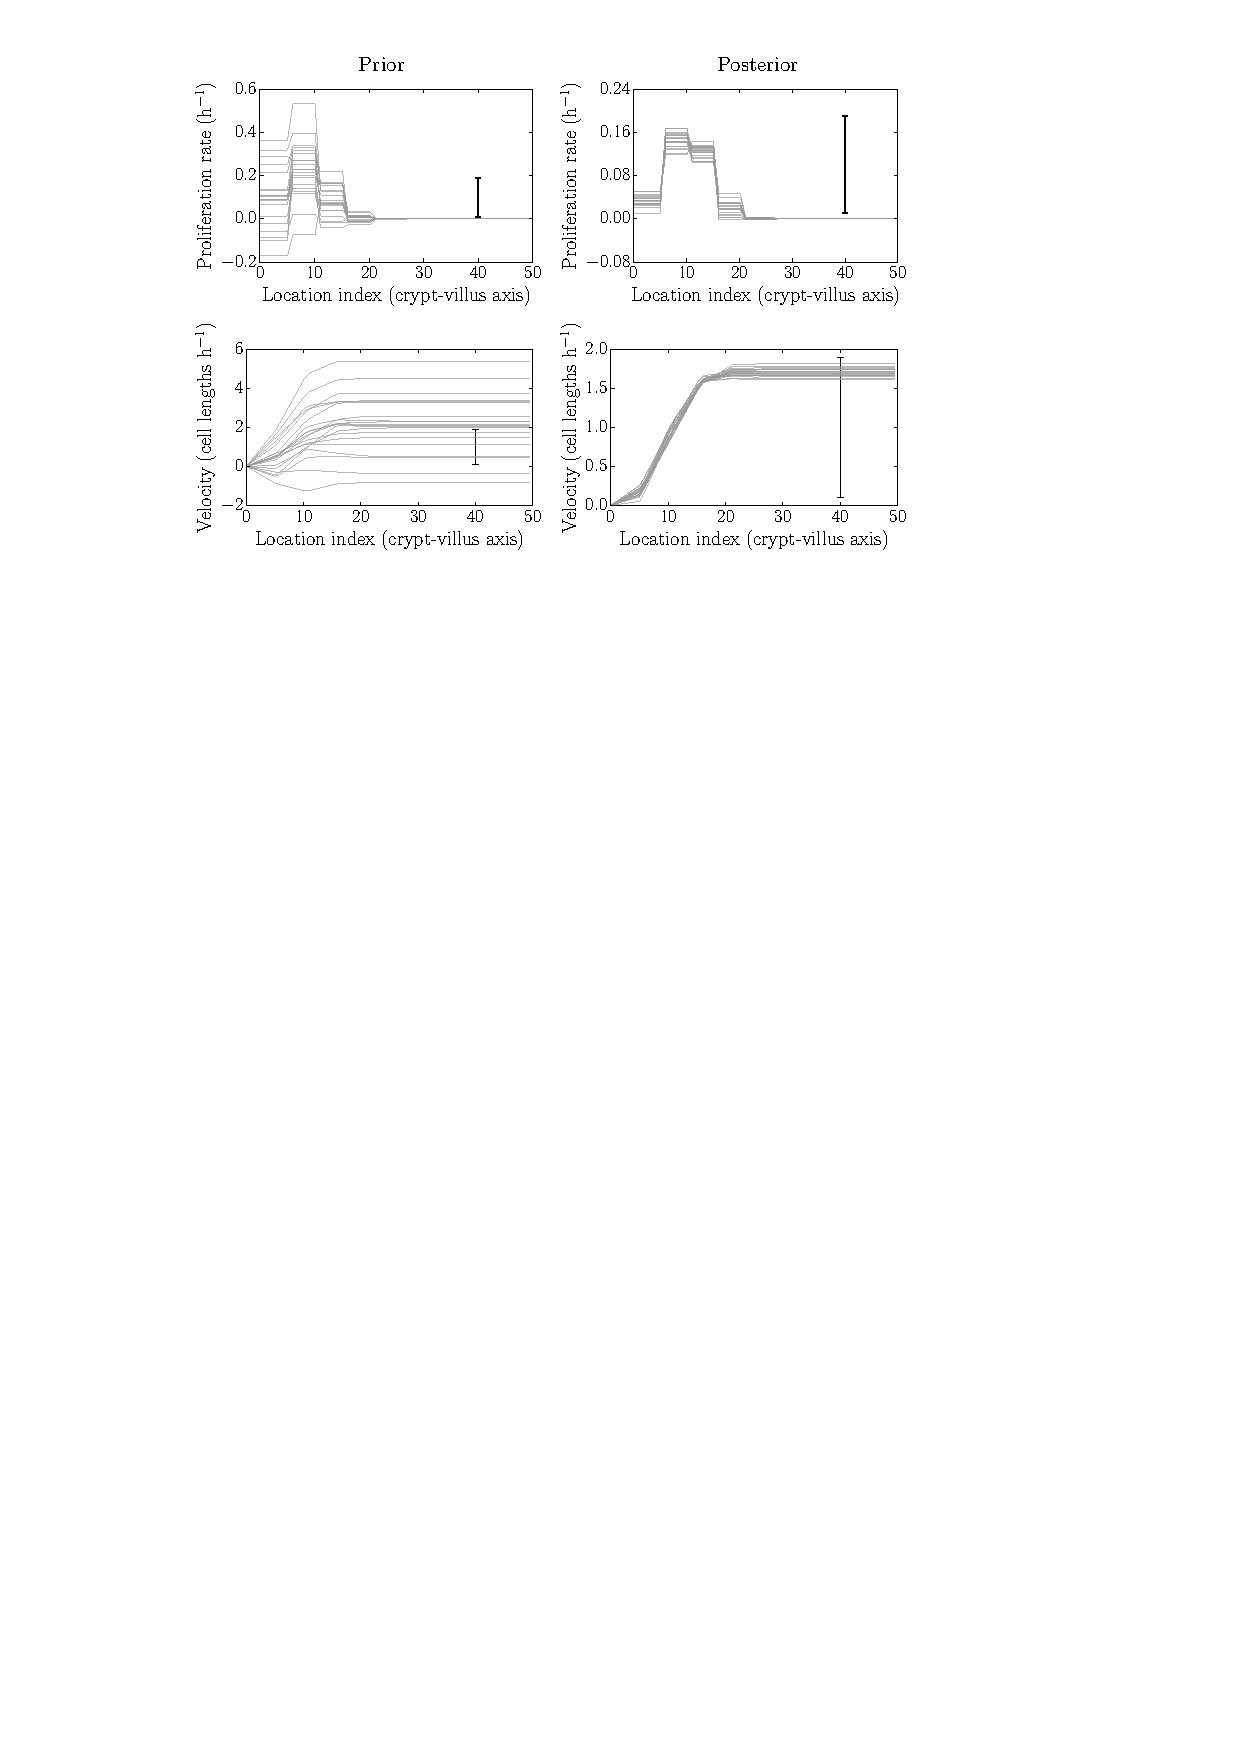
\includegraphics[draft]{../figures/figures_to_include/Fig2}
\caption{Simulated realisations from the prior (left) and posterior
(right) distributions for proliferation profiles (top) and velocities
(bottom). After data are obtained the posterior distributions are much
more tightly-constrained, and are picking out biologically plausible
results (see main text).\label{fig:BrdU-prior-to-posterior-prolif-vel}}
\end{figure}

\subsection{Parameter inference for blocked proliferation
conditions}\label{parameter-inference-for-blocked-proliferation-conditions}

Fig \ref{fig:AraC-prior-to-posterior-prolif-vel} is the same as Fig
\ref{fig:BrdU-prior-to-posterior-prolif-vel} described in the previous
section, but this time under treatment by Ara-C. Results from the
baseline case are shown in grey, while those from Ara-C treatment are
shown in blue. Here 1140 min (19 h post IdU labelling, 2 h post Ara-C
treatment) was used as the initial condition and 1500 min (25 h post IdU
labelling, 8 h post Ara-C treatment) used for fitting. The intermediate
time 1260 min (21 h post IdU labelling, 4 h post Ara-C treatment) and
later time 1620 min (27 h post IdU labelling, 10 h post Ara-C treatment)
were used as out-of-sample comparisons (see later).

\begin{figure}
\centering
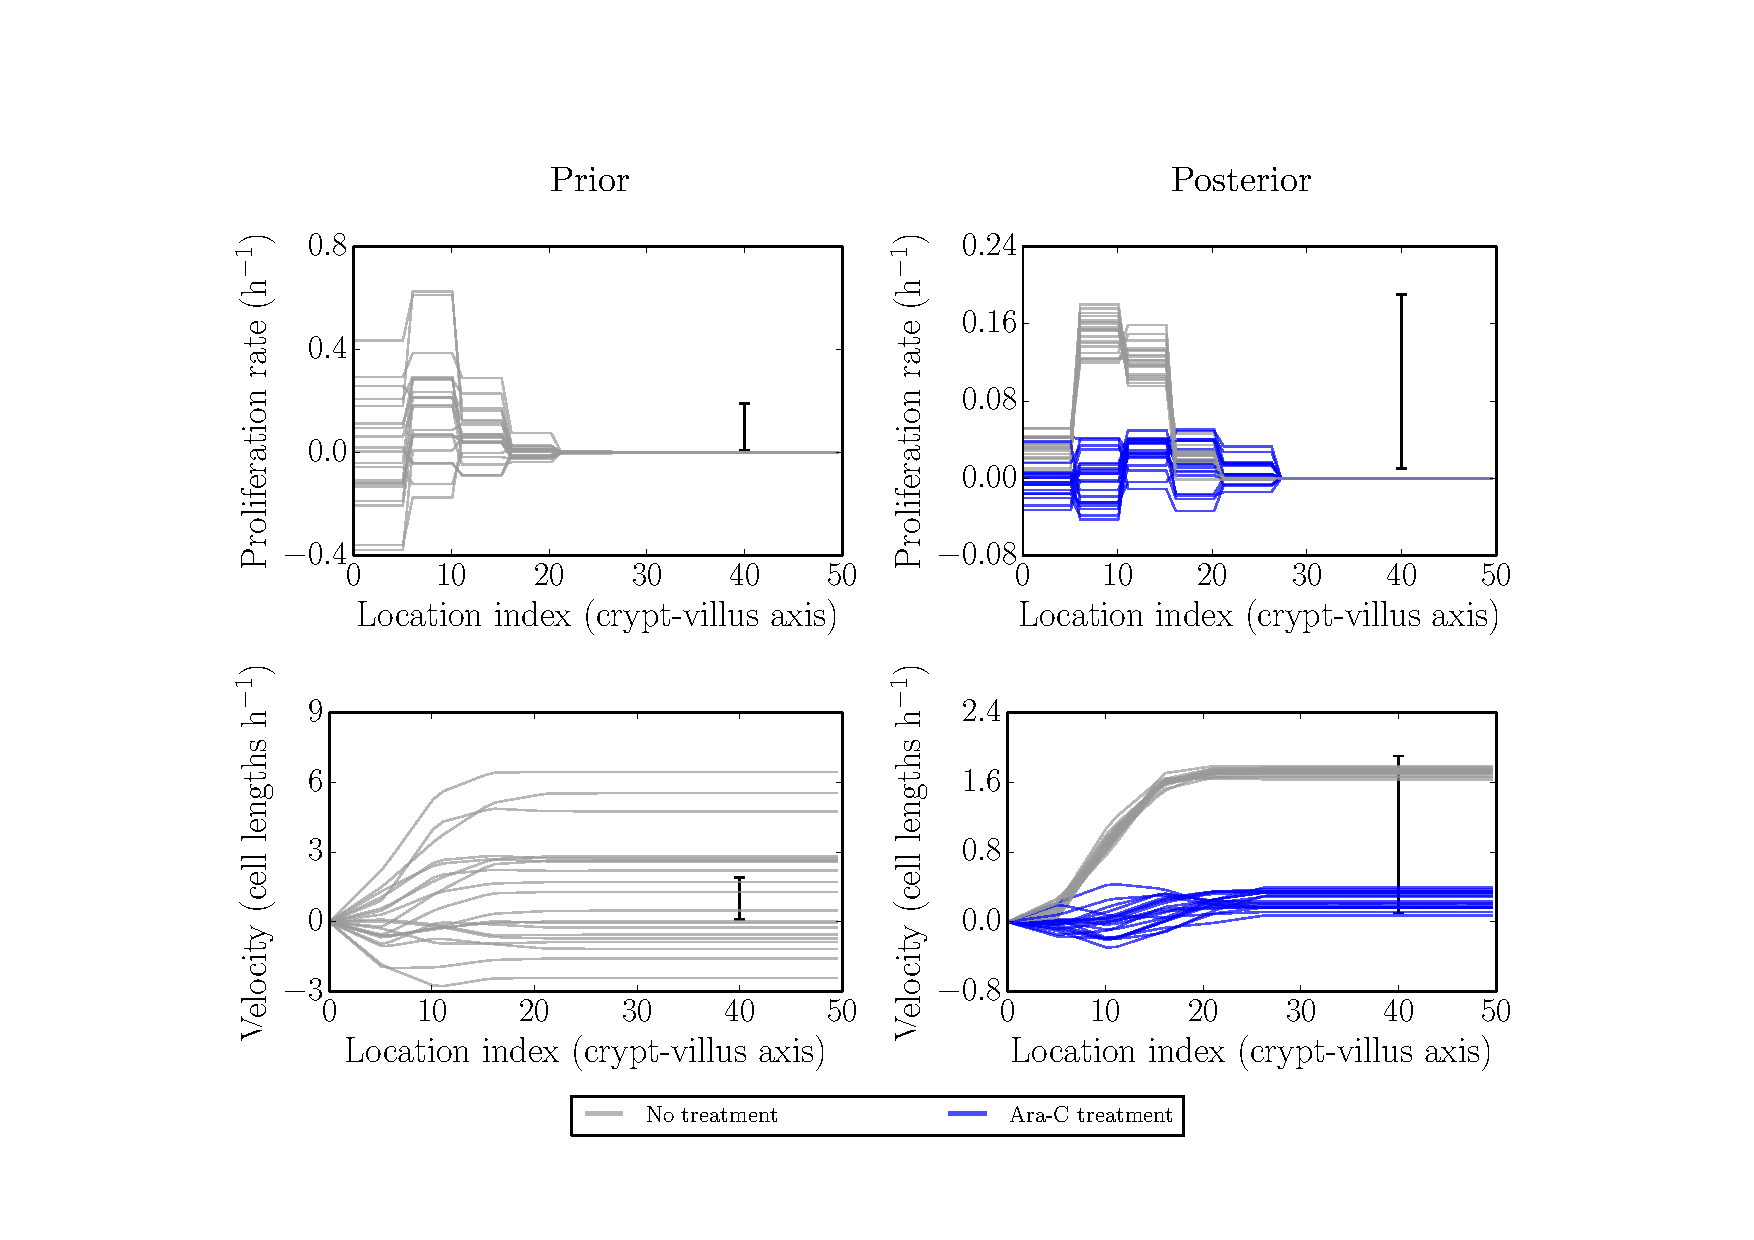
\includegraphics[draft]{../figures/figures_to_include/Fig3}
\caption{Simulated realisations from the prior (left) and posterior
(right) distributions for proliferation profiles (top) and velocities
(bottom) under Ara-C treatment (blue) as compared to no treatment
(grey). The velocities are reduced to near zero, as are the
proliferation rates, though the latter are
noisier.\label{fig:AraC-prior-to-posterior-prolif-vel}}
\end{figure}

As can be seen, there is clear inhibition of proliferation and an even
clearer effect on the cell migration (growth) velocity. The greater
variability in the underlying parameter results compared to the baseline
case may indicate, for example, greater parameter underdetermination
and/or inconsistency of the model. This is not surprising as we expect
all proliferation parameters to be reduced to similar (low) values and
hence to become become less distinguishable.

To add additional stability to the results we can attempt to reduce
underdetermination in the parameters by increasing the parameter
correlation length and inducing an effectively more `lumped'
representation of the parameter field (since values tend to stick
together more). Doing this removed the more extreme negative net
proliferation in the posterior profile, however it still allowed for
small amounts of negative net proliferation/velocity (the available
Jupyter notebook can be used to explore various prior assumptions).

Again, the need to introduce more stability is likely due to some
combination of the limitations of resolution, a consequence of trying to
fit the data too closely, or an indication of model inadequacies. In
particular, under inhibited-proliferation conditions the effective
number of parameters would be expected to be reduced. When fitting the
full model, with largely independent parameters for each region, it is
to be expected that some additional regularisation would be required for
greater stability.

\subsection{Parameter inference for recovering proliferation
conditions}\label{parameter-inference-for-recovering-proliferation-conditions}

Ara-C is metabolised between 10-12 h post-treatment. The two times
considered here, 1620 min and 2520 min, correspond to 10 h and 25 h post
Ara-C treatment, respectively, i.e to the end of the effect and after
the resumption of proliferation. Hence, to check for the recovery of
proliferation, we fitted the model using 1620 min as the initial
condition and 2520 min as the final time.

Fig \ref{fig:AraC-recovery-prior-to-posterior-prolif-vel} is the same as
Fig \ref{fig:BrdU-prior-to-posterior-prolif-vel} and Fig
\ref{fig:AraC-prior-to-posterior-prolif-vel} described in the previous
sections, but this time after/during recovering from treatment by Ara-C.
The previous results from the baseline case are shown in grey, while the
new results following recovery from Ara-C treatment are shown in blue.
Here 1620 min (27 h post IdU labelling, 10 h post Ara-C treatment) was
used as the initial condition and 2520 min (42 h post IdU labelling, 25
h post Ara-C treatment) used for fitting. We did not make additional
out-of-sample comparisons in this case, though in-sample posterior
predictive checks were still carried out (see later).

Here, as expected, the proliferation and velocity profiles indicate that
proliferation has resumed. The rates of proliferation appear to be lower
than under fully healthy conditions, however, perhaps due to incomplete
recovery (the initial condition being right at the beginning of the
recovery period). The timing of the recovery of proliferation and the
well-identified proliferation and velocity profiles inferred give no
indication that any other mechanism is required to account for these
data, however.

\begin{figure}
\centering
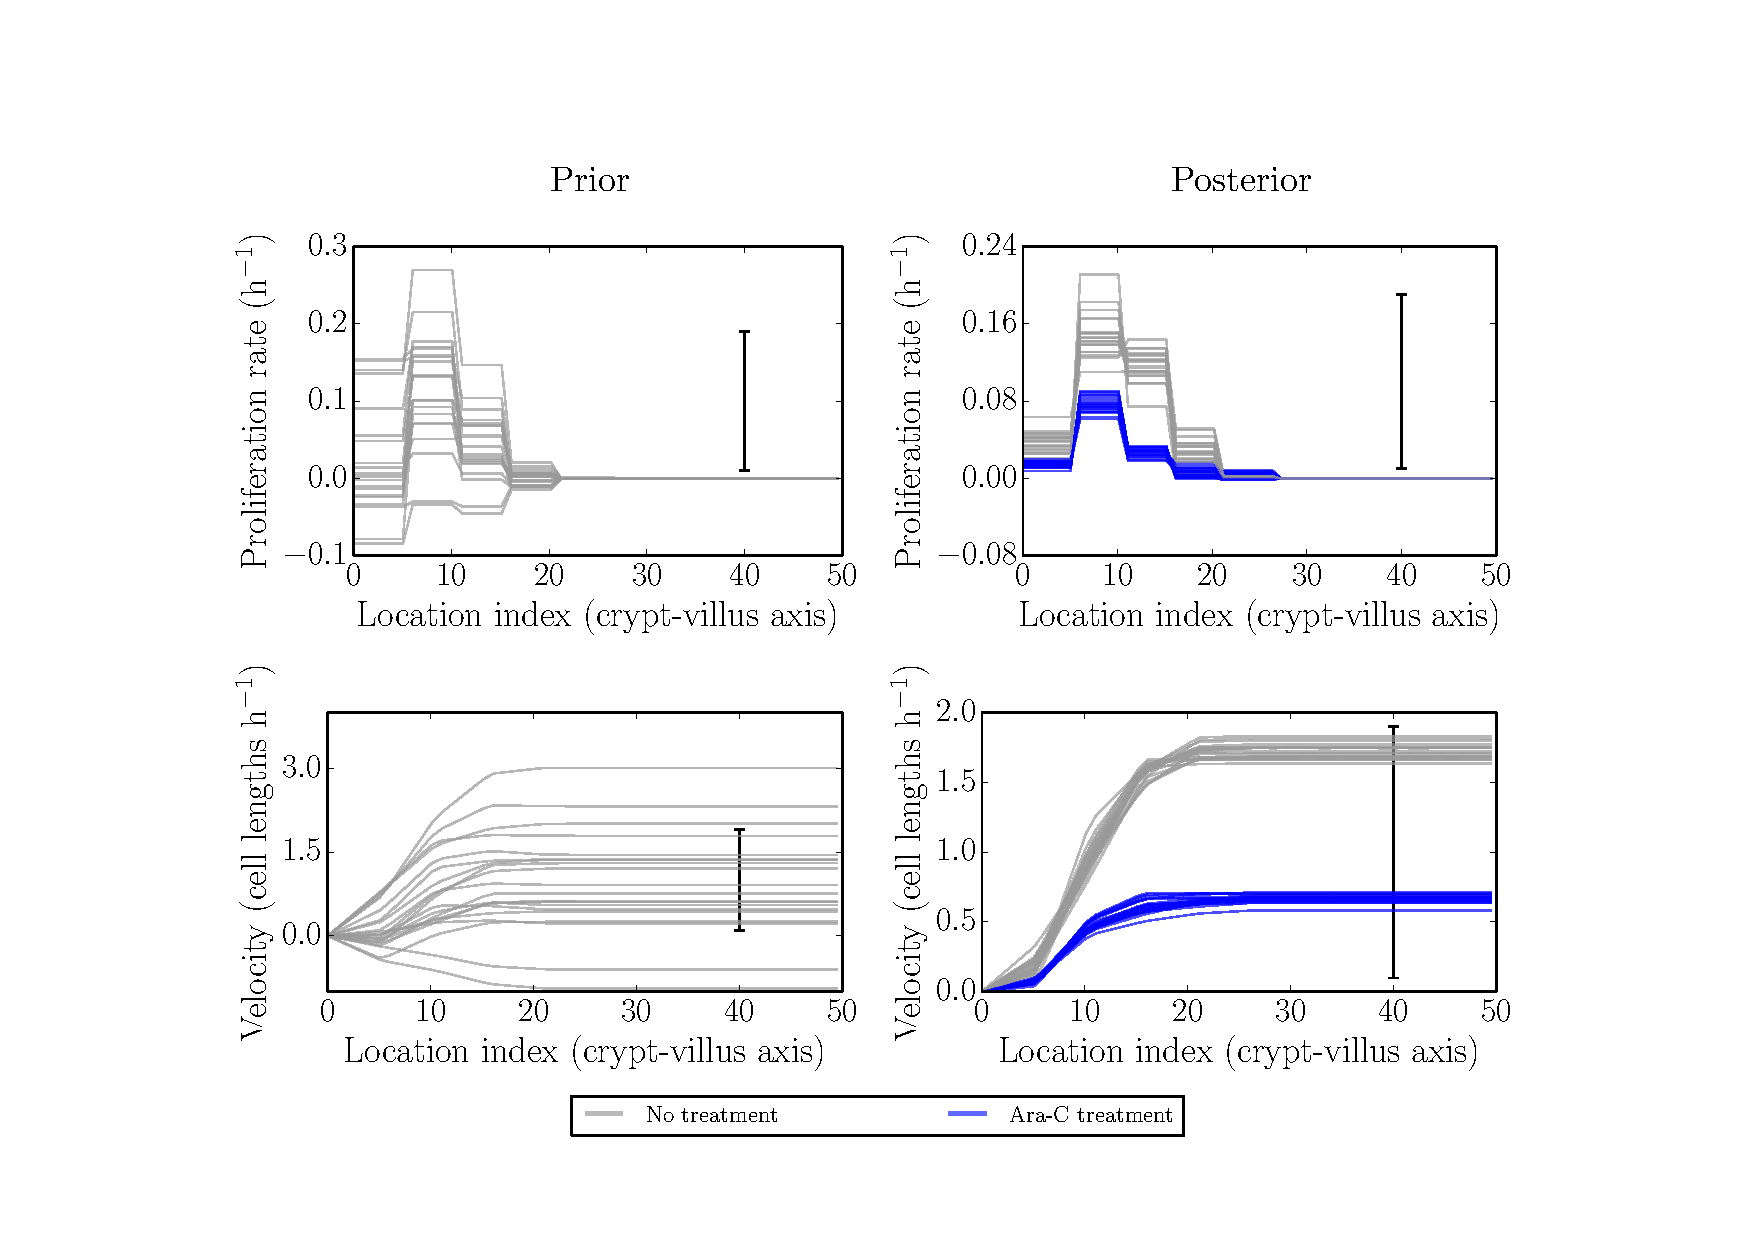
\includegraphics[draft]{../figures/figures_to_include/Fig4}
\caption{Simulated realisations from the prior (left) and posterior
(right) distributions for proliferation profiles (top) and velocities
(bottom) after recovery from Ara-C treatment (blue) as compared to no
treatment (grey). The velocities and proliferation rates show partial
recovery towards healthy
conditions.\label{fig:AraC-recovery-prior-to-posterior-prolif-vel}}
\end{figure}

\subsection{Predictive checks under homeostatic (healthy)
conditions}\label{predictive-checks-under-homeostatic-healthy-conditions}

Fig \ref{fig:BrdU-prior-to-posterior-label} illustrates simulations from
the predictive distributions corresponding to the prior and posterior
parameter distributions of Fig
\ref{fig:BrdU-prior-to-posterior-prolif-vel}. This enables a first
self-consistency check - i.e.~can the model re-simulate data similar to
that to which it was fitted {[}20, 58{]}? If this is the case then we
can (provisionally) trust the parameter estimates in the previous
figure; if not, then the parameter estimates would be unreliable, no
matter how well-determined they seem. In our case the model appears to
adequately replicate the data used for fitting.

\begin{figure}
\centering
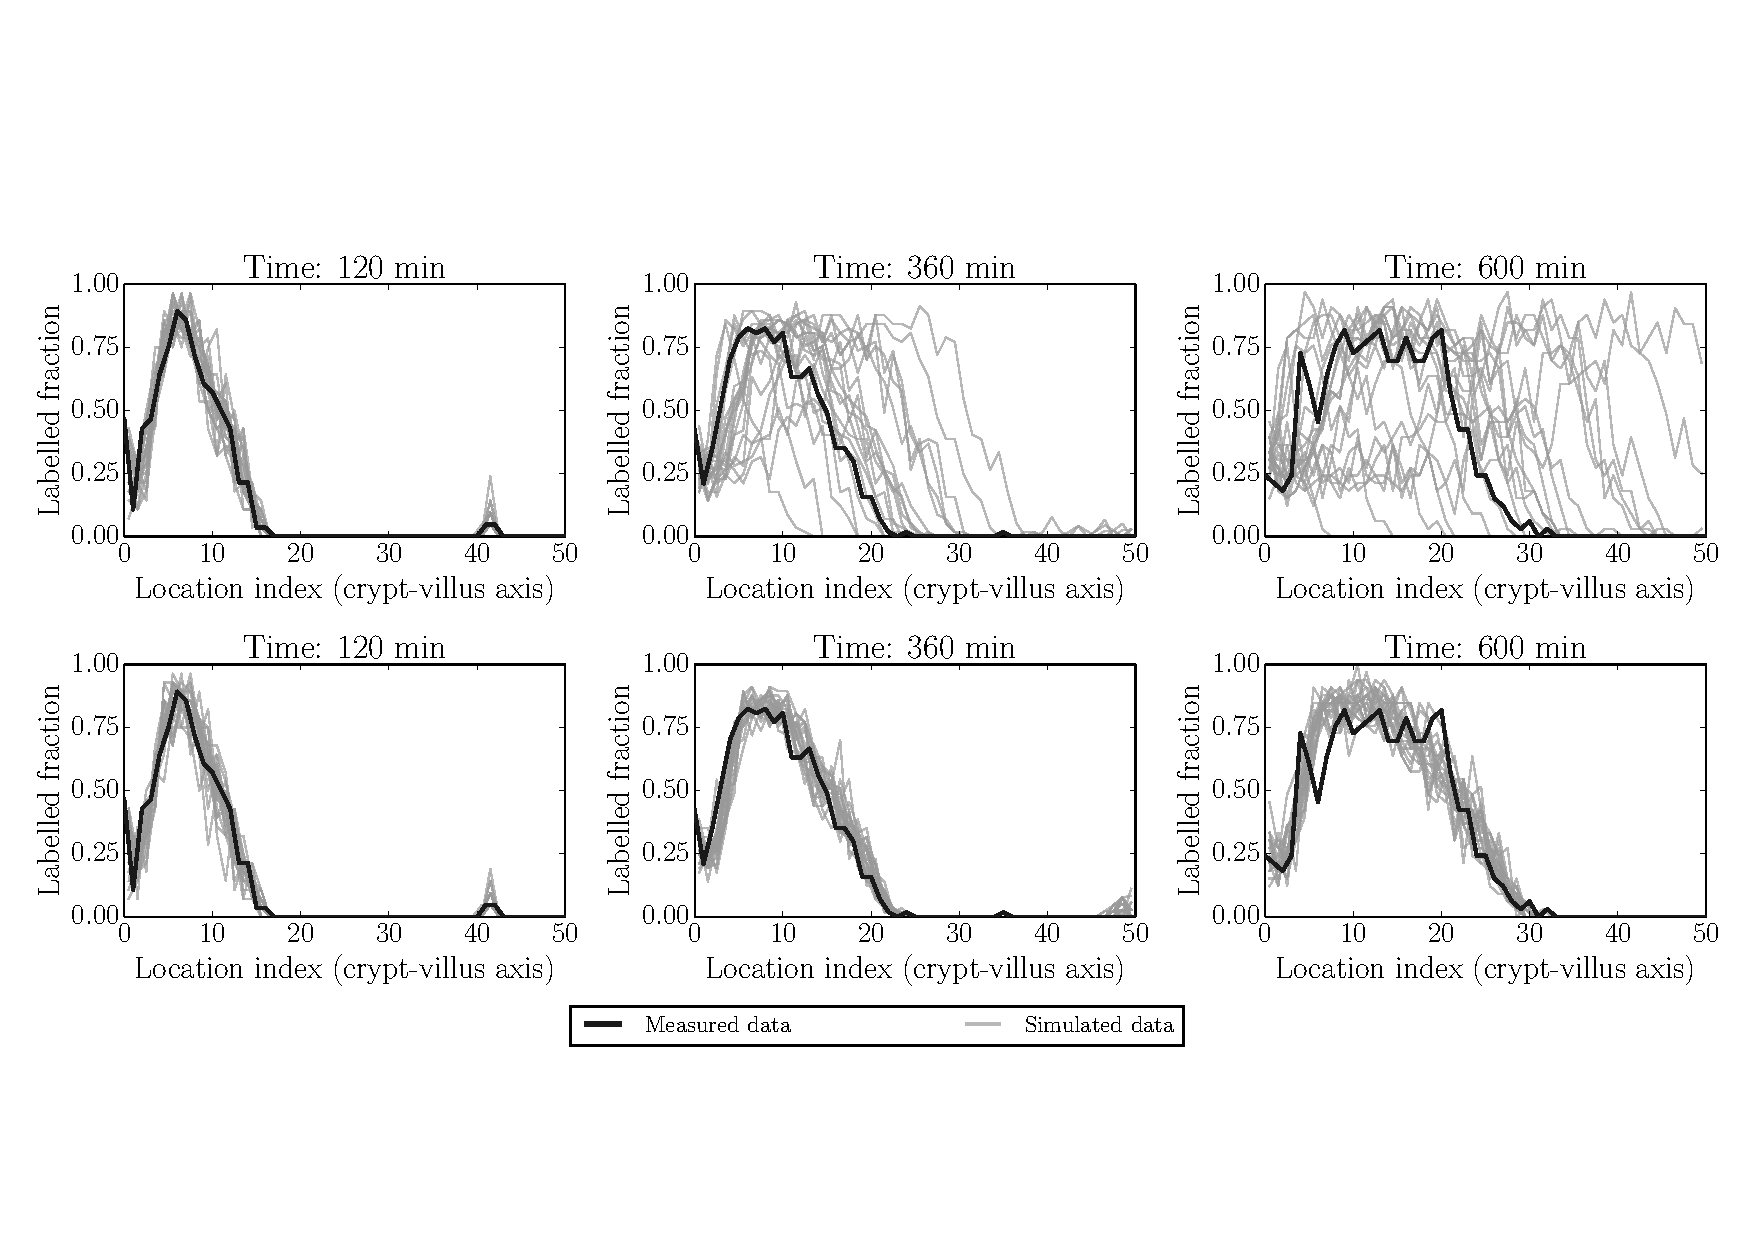
\includegraphics[draft]{../figures/figures_to_include/Fig5}
\caption{Simulated realisations from prior (top) and posterior (bottom)
predictive distributions (grey) for label data at fitted times (120 min,
360 min and 600 min i.e.~2 h, 6 h and 10 h). Actual data are indicated
by black lines. Again the posterior distributions are much more
constrained than the prior distributions, representing the gain in
information from collecting (and fitting to) experimental data. The
first profile in each panel is held as a constant initial condition in
this example.\label{fig:BrdU-prior-to-posterior-label}}
\end{figure}

Fig \ref{fig:BrdU-future-realisations-1080-min} and Fig
\ref{fig:BrdU-posterior-characteristics} illustrate two additional ways
of visualising replicated datasets. The former visualises the label
profile along the crypt-villus axis at the future unfitted/out-of-sample
time 1080 min (18 h), while the latter visualises both fitted (120 min/2
h, 360 min/6 h and 600 min/10 h) and unfitted/out-of-sample (1080 min/18
h) predictions plotted in the characteristic plane \((t,x)\) in which
the slopes along lines of constant colour should be inversely
proportional to the migration velocities at that point, due to the
(hyperbolic) nature of our `colour' equation (see e.g. {[}59{]}). We
have interpolated between the dotted grid lines. These figures, in
combination with Fig \ref{fig:BrdU-prior-to-posterior-label} above,
indicate that the model is capable of reliably reproducing the data to
which it was fitted, as well as predicting key features of unfitted
datasets such as the rate of movement of the front. On the other hand,
there is clearly a greater misfit with the predicted rather than fitted
data. In order to locate the possible source of misfit we considered
various model residuals and error terms - see `Locating model misfit'
below.

\begin{figure}
\centering
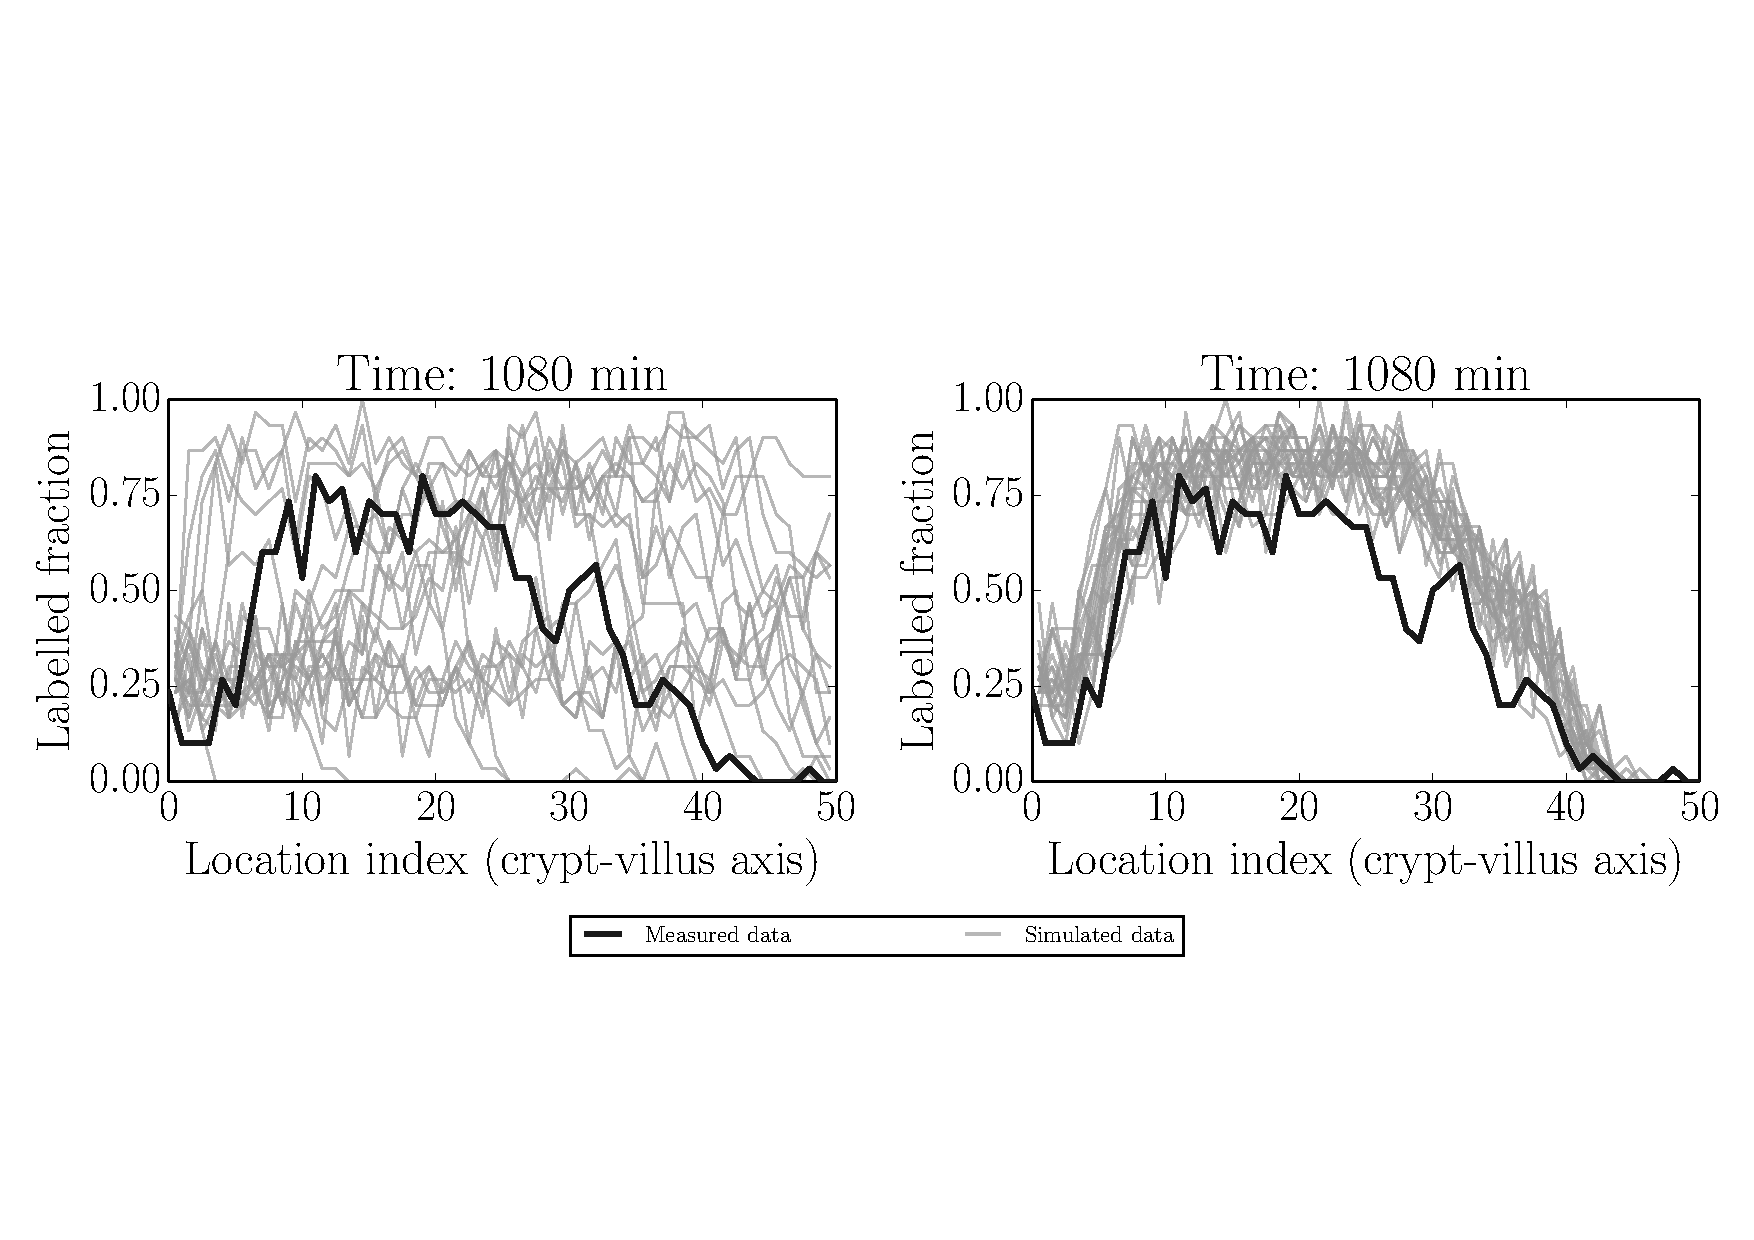
\includegraphics[draft]{../figures/figures_to_include/Fig6}
\caption{Simulated realisations from prior (left) and posterior (right)
predictive distributions (grey) for label data at the unfitted
(out-of-sample) time 1080 min (18 h). Actual data are indicated by black
lines. The model appears to give reasonable predictions capturing the
key features, but there is also some misfit to be explored
further.\label{fig:BrdU-future-realisations-1080-min}}
\end{figure}

\begin{figure}
\centering
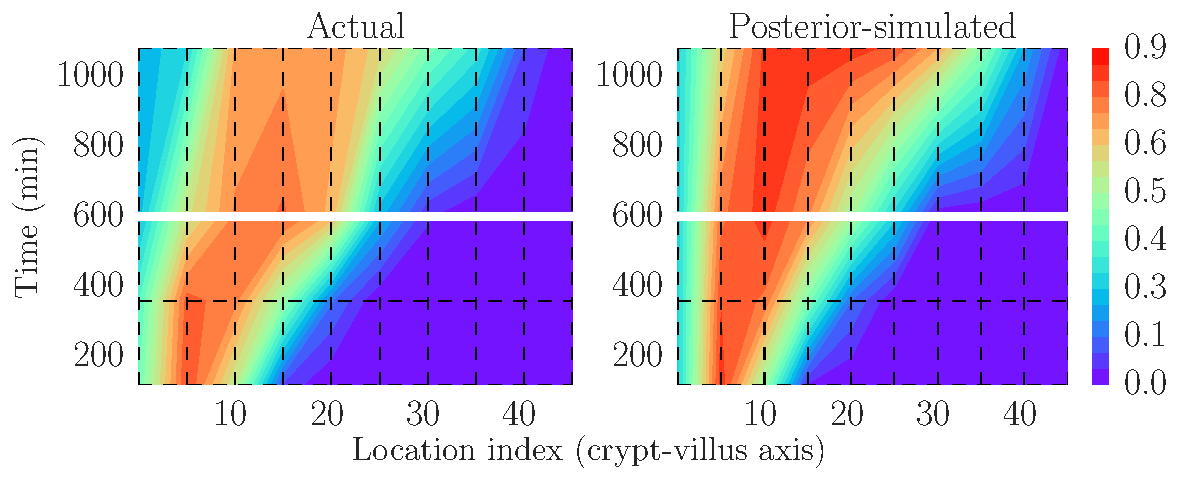
\includegraphics[draft]{../figures/figures_to_include/Fig7}
\caption{Actual (smoothed) data (left, black box) and one replication
based on the model (right; plotting the latent/measurement-error-free
process) as visualised in the characteristic plane. This has been
discretised and interpolated between the dotted lines to facilitate fair
but coarse-grained comparisons. The model structure implies that there
should be lines of constant colour tracing out curves with slopes
inversely proportional to the migration velocities at that point. The
model again captures several of these key qualitative features, but fits
less well for the out-of-sample (above the horizontal gap at 600 min/10
h) data. There is little variability in the latent model process and so
only one replication is
shown.\label{fig:BrdU-posterior-characteristics}}
\end{figure}

\subsection{Predictive checks under blocked proliferation
conditions}\label{predictive-checks-under-blocked-proliferation-conditions}

Here data from 1140 min (19 h; post IdU labelling) were used as the
initial conditions and 1500 min (25 h) used for fitting. 1260 min (21 h)
and 1620 min (27 h) were used as out-of-sample (non-fitted) comparisons.
Fig \ref{fig:AraC-posterior-label-all} is analogous to Fig
\ref{fig:BrdU-prior-to-posterior-label} in the healthy case. In general
all of the features up to 1620 min (27 h) in Fig
\ref{fig:AraC-posterior-label-all}, and for both fitted and predicted
times, are reasonably well captured. The fit at 1620 min is generally
good, but perhaps worse than the other cases. This could be due to
errors in longer-time predictions and to the beginning of proliferation
recovery: we explore these alternatives in what follows.

\begin{figure}
\centering
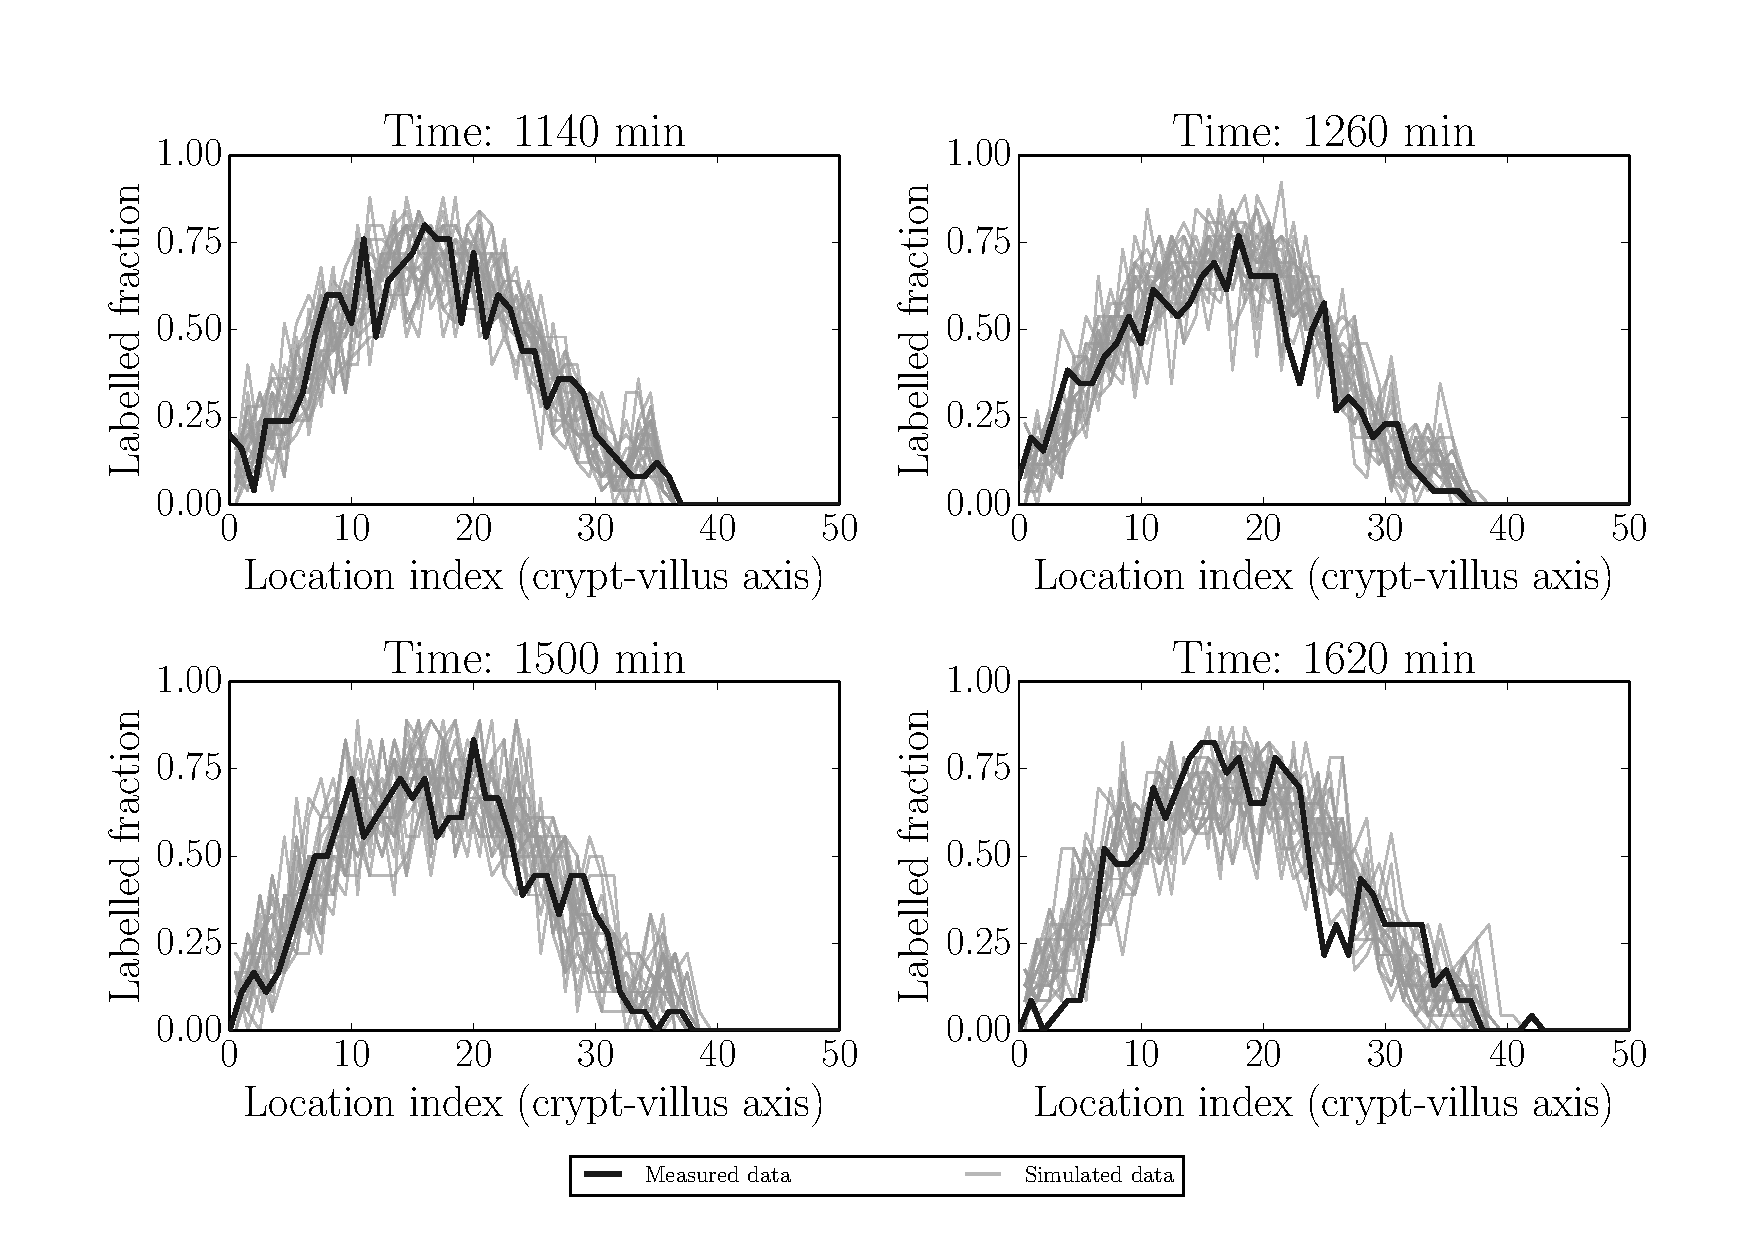
\includegraphics[draft]{../figures/figures_to_include/Fig8}
\caption{Simulated realisations from posterior predictive distributions
(grey) for label data at 1140 min (initial condition), 1500 min (fitted
time) and at two out-of-sample/unfitted times (1260 and 1620 min). The
posterior distributions appear to adequately capture the actual label
data (black).\label{fig:AraC-posterior-label-all}}
\end{figure}

\subsection{Predictive checks under recovering proliferation
conditions}\label{predictive-checks-under-recovering-proliferation-conditions}

As discussed above, Ara-C is metabolised between 10-12 h post-treatment.
The two times considered here, 1620 min and 2520 min, correspond to 10 h
and 25 h post Ara-C treatment, respectively, i.e to the end of the
effect and after the resumption of proliferation.

Again, as expected, the label has resumed movement in concert with the
resumption in proliferation. The model appears to fit reasonably well.

\begin{figure}
\centering
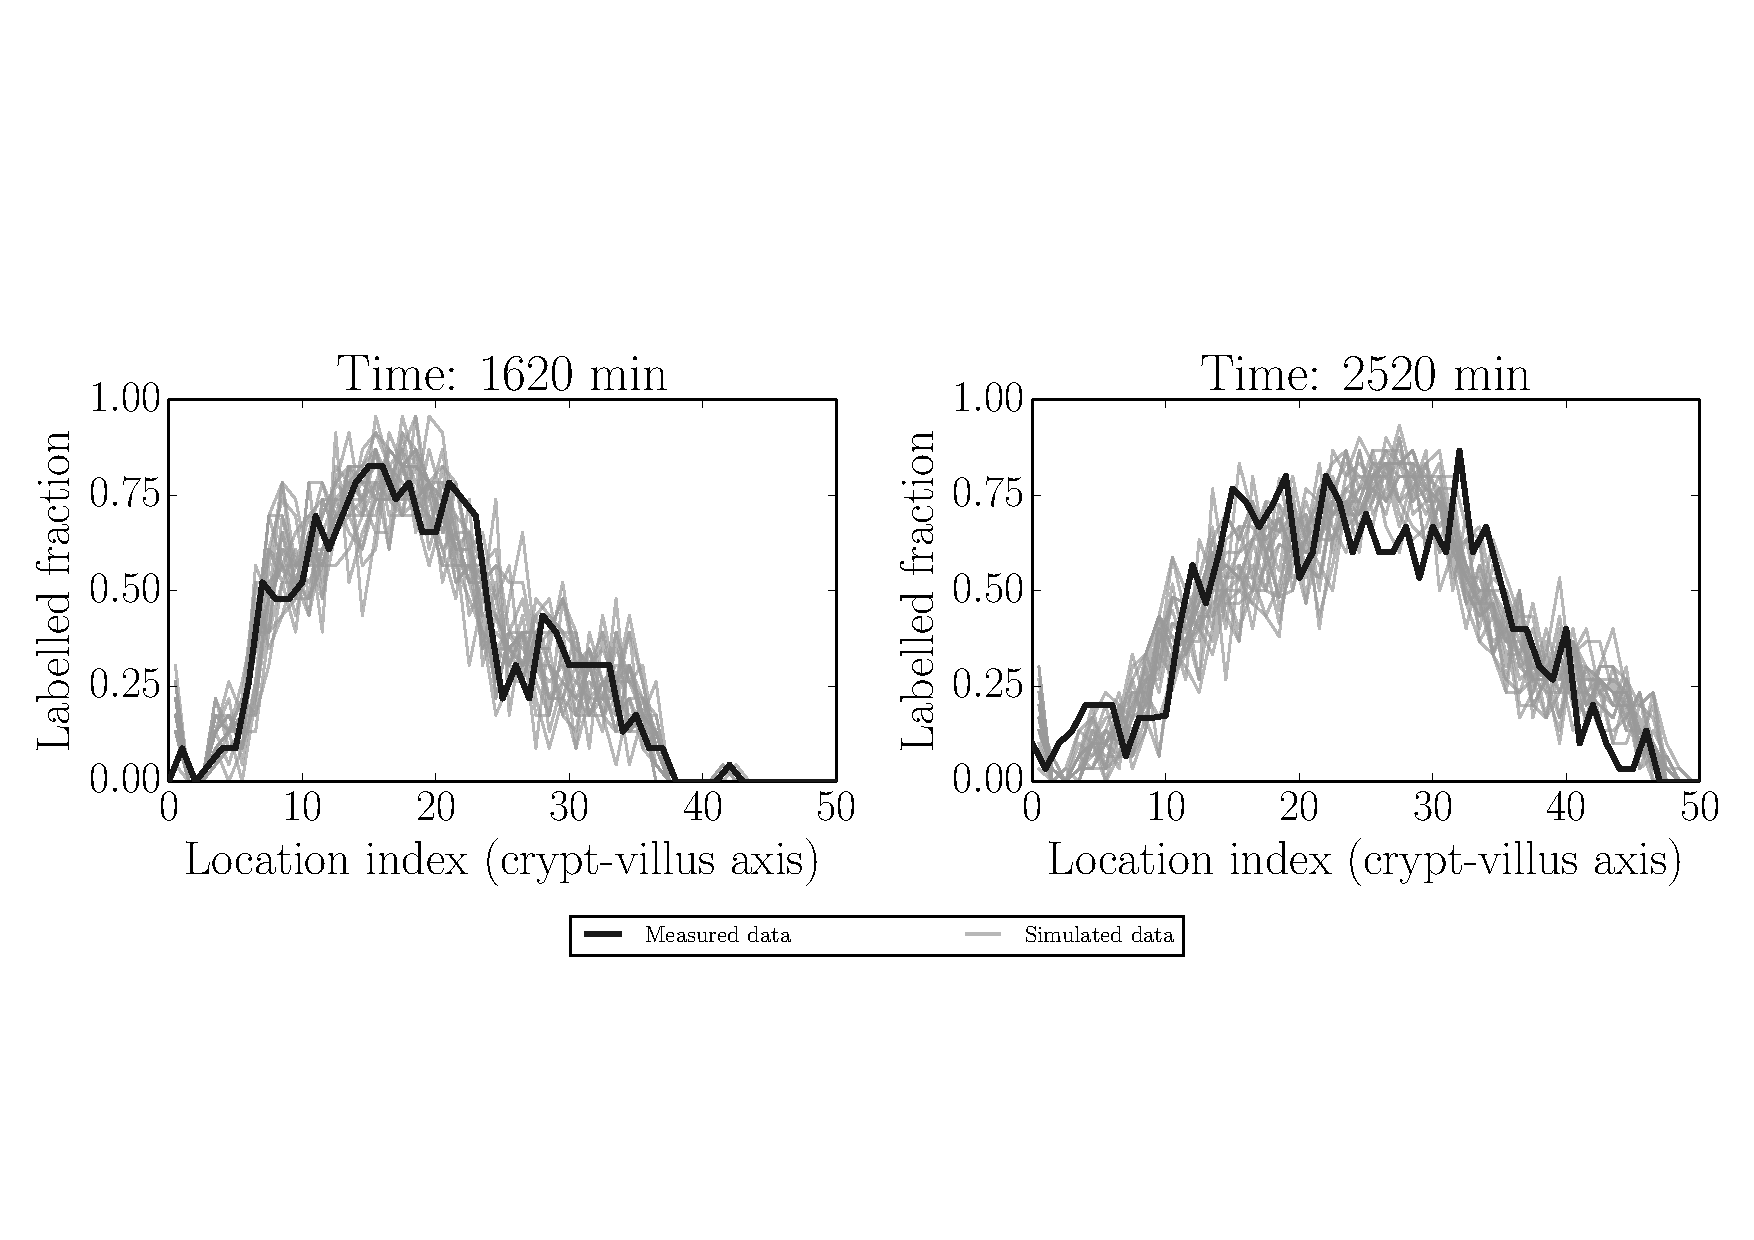
\includegraphics[draft]{../figures/figures_to_include/Fig9}
\caption{Simulated realisations from posterior predictive distributions
(grey) for label data at 1620 min (initial condition) and 2520 min
(fitted). These indicate that proliferation has resumed, consistent with
the time taken to metabolise Ara-C - see the main text for more
detail.\label{fig:AraC-recovery-posterior-label-all}}
\end{figure}

\subsection{Locating model misfit}\label{locating-model-misfit}

While the zeroth-order model behaves essentially as desired under
experimental perturbation, and is likely capturing the essential
features of interest, we observed some minor model misfit. We used
posterior predictive checks to unpick the contributions of the various
model parts and determine the source(s) of misfit. This in turn
motivated potential model improvements. These checks were carried out
under baseline (healthy) conditions as we were more confident of the
experimental effects under this scenario, but they can equally be
carried out for the other datasets. Note, however, that time-varying
effects are not expected to be as relevant under conditions of inhibited
proliferation.

Fig \ref{fig:BrdU-posterior-residuals} shows the following checks:
measurement error as determined by subtracting a smoothed spline from
the observed data (dark line) and comparing these to the results
obtained by subtracting the process model from the simulated data
(panels 1-4, moving left-to-right and top-to-bottom, showing fitted -
120 min/2 h, 360 min/6 h and 600 min/10 h - and unfitted/out-of-sample -
1080 min/18 h - times). This presentation follows the noise-checking
approach in {[}60{]}, as well as the general recommendations given in
{[}20, 58{]}. Reliable interpretation of these as `true' measurement
residuals depends on the validity of the normal approximation
\ref{eq:likel-norma} since these expressions are not directly
interpretable in terms of the discrete binomial model (see e.g. {[}20,
58{]}). These are also visualised in terms of the corresponding
cumulative distributions in the middle panel (panel 5, following as
above). Panels 6-9 show the differences between the underlying process
model and the smoothed spline fitted to the data. As can be seen, the
measurement model appears approximately valid at all times, while the
process model appears to have non-zero error for the 1080 min sample. We
consider this in more detail next.

\begin{figure}
\centering
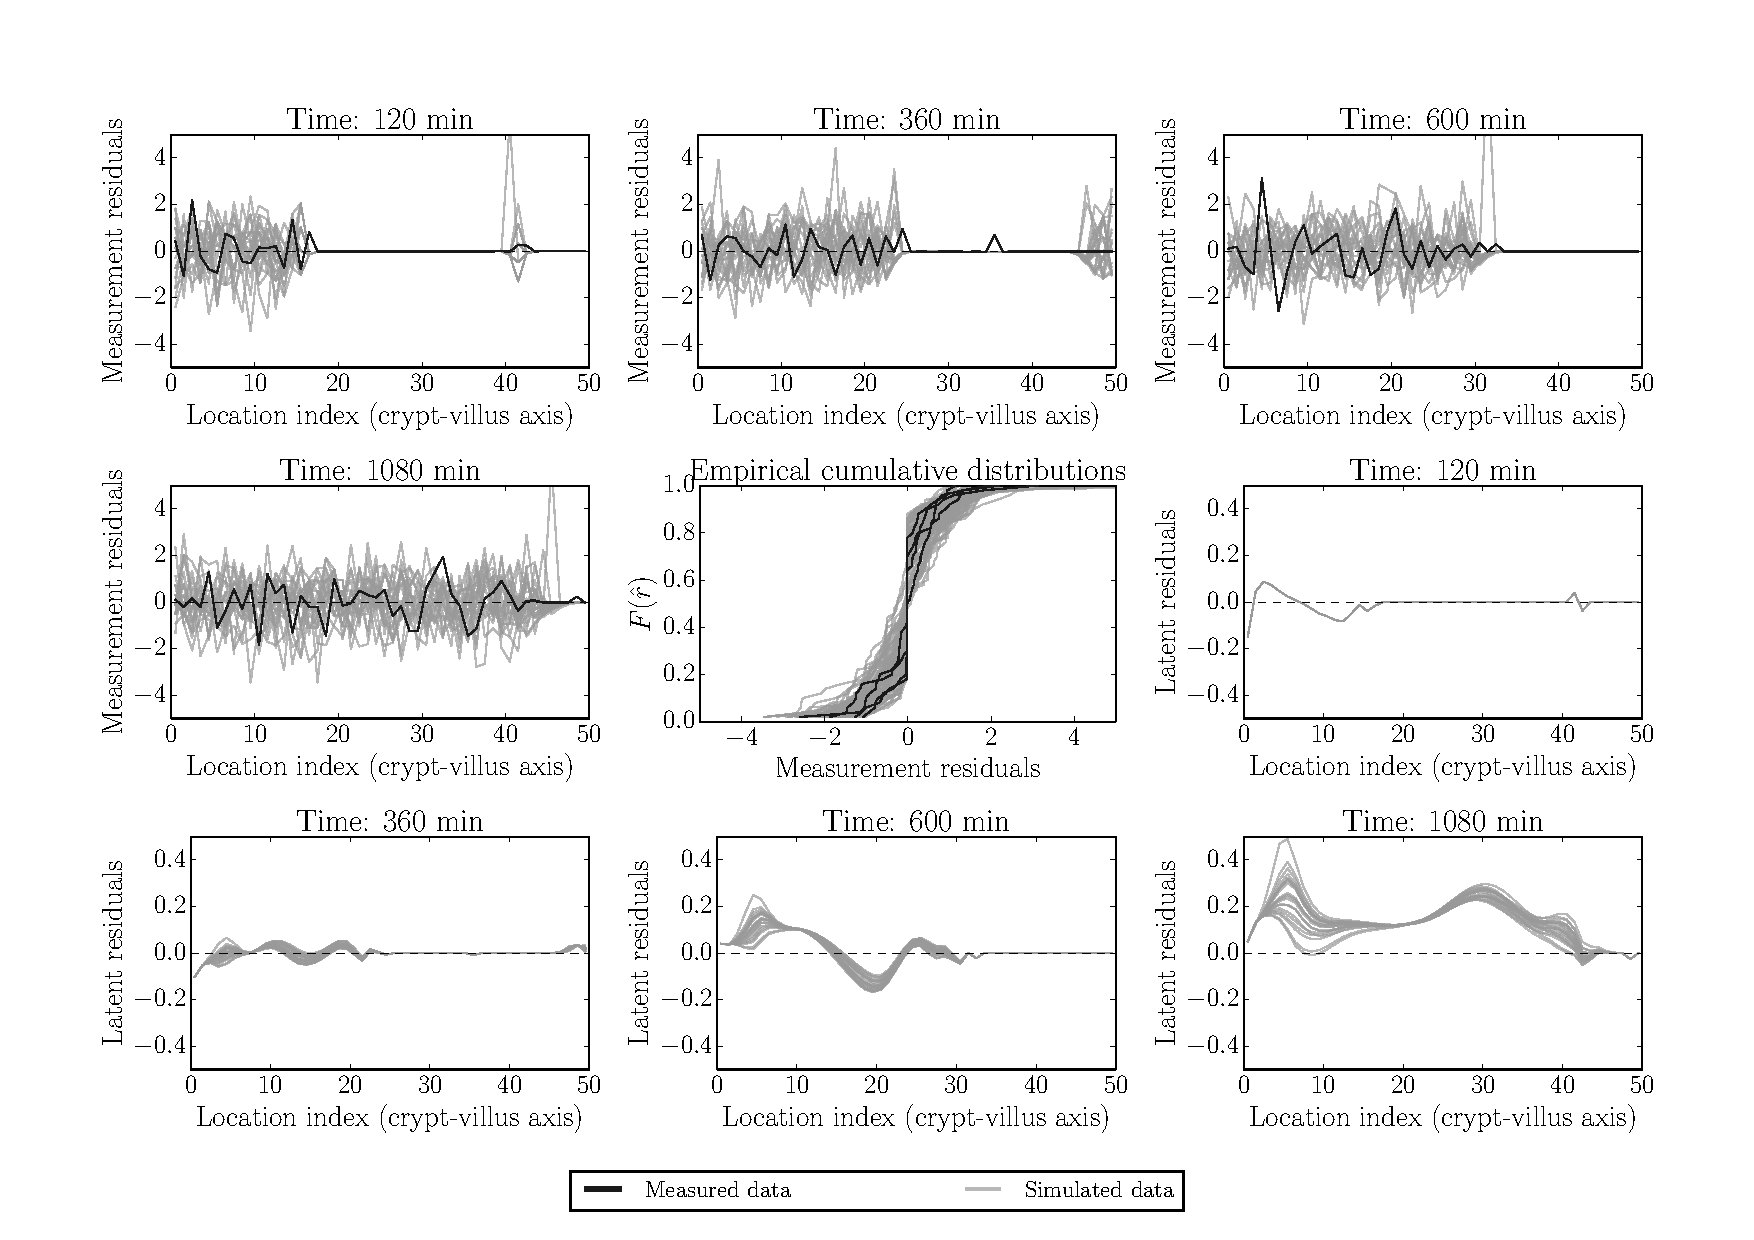
\includegraphics[draft]{../figures/figures_to_include/Fig10}
\caption{Model and data residual components. Panels 1-4, moving
left-to-right and top-to-bottom, shows measurement error as determined
by subtracting a smoothed spline from the observed data (dark line) and
comparing this to the results obtained by subtracting the process model
for fitted - 120, 360 and 600 mins - and unfitted/out-of-sample - 1080
min - times from the realised data (grey). These measurement error
distributions are also visualised in terms of the corresponding
cumulative distributions in the middle panel (panel 5, following as
above. Black - actual data, grey - model simulations). Panels 6-9 show
the differences between realisations of the underlying process model and
the smoothed spline fitted to the data. As can be seen across panels,
the measurement model appears approximately valid at all times, while
the process model appears to have non-zero error for the 1080 min
sample. This observation is discussed in the
text.\label{fig:BrdU-posterior-residuals}}
\end{figure}

\subsection{Possible model improvement and robustness - higher-order
spatial
effects}\label{possible-model-improvement-and-robustness---higher-order-spatial-effects}

As discussed in the process model section above, the presence of
cellular structure in the epithelial tissue means that higher-order
spatial effects could be present. One way of deciding whether these are
important is to consider the extent to which these may account for the
minor misfit identified above, as opposed to other factors such as
time-varying proliferation rates. To do this we considered both uniform
percentage reductions of the original parameter estimates (approximating
time-varying rates) and the inclusion of higher-order spatial terms.

Fig \ref{fig:BrdU-comparison-diffusion-correction} gives an idea of the
qualitative differences induced by including the higher-order spatial
terms and those that could be induced by time-varying proliferation
rates. This figure is based on the (healthy) 1080 min (18 h) data in
which we found some indication of a process model error.

We see that while the higher-order model appears to give a slightly
better qualitative fit to the data, both the higher-order and
lower-order models require similar reductions of the parameter values to
quantitatively improve the fit to our out-of-sample data. The reduced
parameter values shown in Fig
\ref{fig:BrdU-comparison-diffusion-correction} correspond to a reduction
of 20\%, which was chosen visually as a reduction accounting for the
bulk of the misfit.

Thus the key (yet relatively small) difference between the model and
out-of-sample data is likely due to an effect other than finite-cell
sizes; in this case it is likely due to time-variation in parameter
values due to circadian rhythms (we have assumed steady-state parameter
values). Other potential factors include label dilution or an unmodelled
mixing phenomenon in the full two-dimensional case. We note however that
these effects are small and appear to be important primarily for
predicting much further ahead in time than the fitted data and the
steady-state parameter assumption is likely valid for reasonable time
intervals. This means that the more easily interpretable original model
may be sufficient for many purposes.

\begin{figure}
\centering
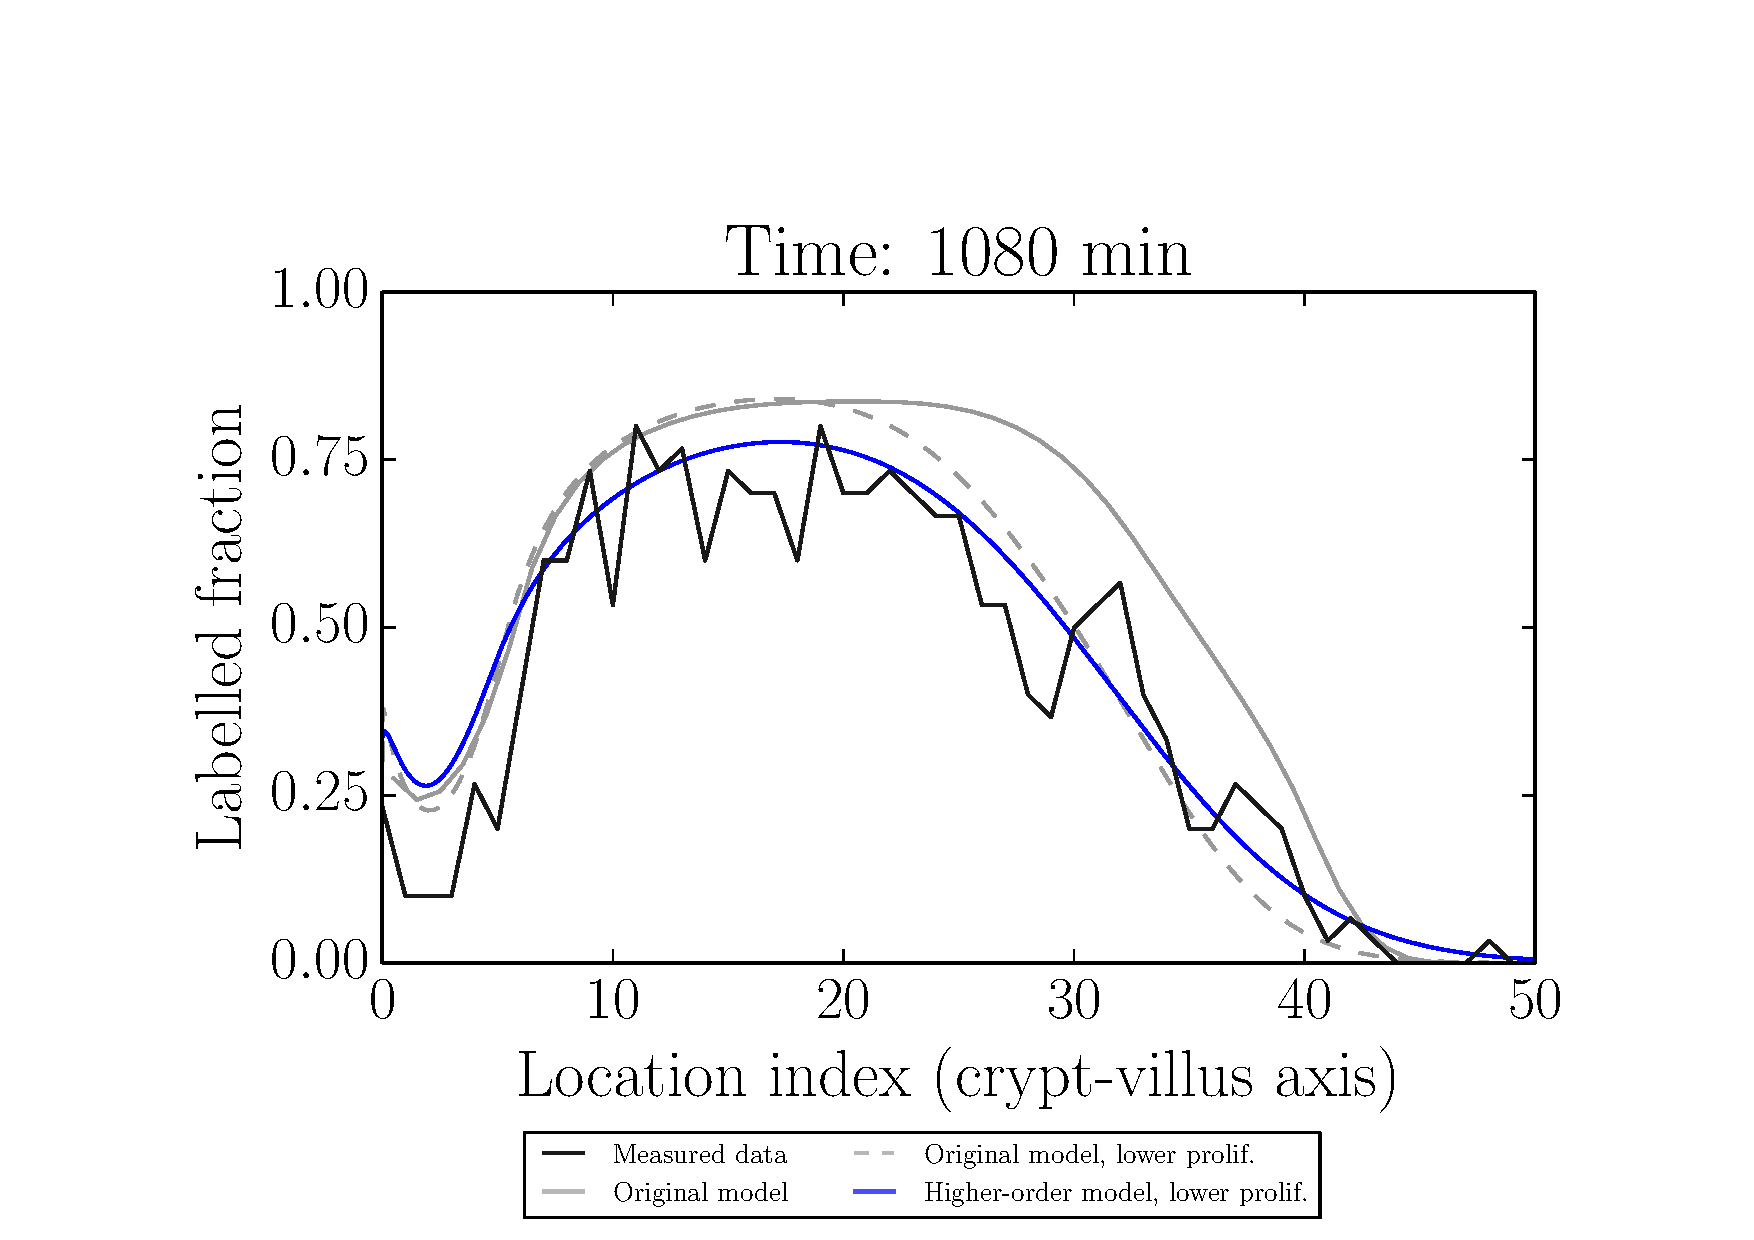
\includegraphics[draft]{../figures/figures_to_include/Fig11}
\caption{Comparison of the modified process model which includes
higher-order spatial terms (blue) to the original model (grey, dashed),
both at lowered proliferation rates (decreased 20\%), which is required
for a better fit to the data. The original model at the original fitted
proliferation rates is also shown (grey, solid). Although the model with
higher-order spatial terms gives a better qualitative fit to the data
for the same proliferation rates, it is clear that the dominant cause of
misfit is better attributed to (time) varying proliferation rates (in
the context of the present set of
models).\label{fig:BrdU-comparison-diffusion-correction}}
\end{figure}

\section{Discussion}\label{discussion}

Understanding the intricate dynamics of the intestinal epithelium
requires an interdisciplinary approach that integrates experimental
measurements, mathematical and computational modelling, and statistical
quantification of uncertainties. While a diverse range of mathematical
models have been proposed for epithelial cell and tissue dynamics
(reviewed in {[}51, 52, 61--63{]}), from compartment models to
individual-based models to continuum models, we lack consistent and
reproducible approaches for comparing models representing conjectured
biological mechanisms both to each other and to experimental data (for
an overview, see our review {[}44{]}). These shortcomings may explain
why questions such as the connection between proliferation and migration
and its variation under experimental perturbations remain open
{[}8--14{]}.

The aim of the present work was to acknowledge and confront these
difficulties explicitly, and to present some initial constructive steps
towards establishing such a framework. To do this we carried out new
experiments (described more fully in a companion paper {[}18{]}) aimed
at determining how cell proliferation rates, tissue growth and cell
migration rates are related in the intestinal epithelium under healthy,
damaged (Ara-C treated) and recovering conditions. We performed BrdU/IdU
cell-labelling experiments under these respective conditions. We then
developed a probabilistic, hierarchical (conditional) model to process
and interpret these data.

Our hierarchical model provides a best-practice approach for describing
and understanding the uncertainties that could lead to unreliable
mechanistic conclusions - uncertainties in experimental measurement and
treatment, difficult-to-compare mathematical models of underlying
mechanisms, and unknown or unobserved parameters. Our approach was
influenced by recognising the benefits that the hierarchical Bayesian
approach has demonstrated in applications across a number of different
disciplines (e.g.~in environmental and geophysical science as in {[}64,
65{]}; ecological modelling as in {[}66, 67{]}; and in Bayesian
statistical modelling and inverse problems more generally as in
{[}20--24, 68{]}). We also note that a hierarchical approach can have
significant benefits outside the Bayesian framework (see for example the
`extended likelihood' approach described in {[}69--71{]}).

The hierarchical approach provides a framework, not only for combining
disparate sources of uncertainty, but also for facilitating modelling
derivations and relating discrete and continuous models. Though the
resulting measurement, process and parameter models can be (or have
been) derived by other means, as far as we are aware this particular
perspective has not been systematically utilised in the manner
considered here.

We also note the connection between the choice of a measurement model as
required here (and/or process model error, and following e.g. {[}21--24,
64, 72{]}), and the development of approximate sampling and parameter
fitting procedures, which are particularly useful for analytically
difficult models. A key concern of the latter is the appropriate choice
of summary statistics for constructing a `synthetic likelihood' {[}73{]}
or similarly-modified posterior target for Approximate Bayesian
Computation (ABC) {[}74--76{]}. This choice determines (implicitly or
explicitly) in which ways a given model or set of models can be
considered an `adequate' representation of the data, which features are
considered to be reproducible and what the associated `noise' structure
should be ({[}77{]} presents an alternative approach to characterising
data features and model adequacy). These issues are crucial in deciding
how to model the complexity of epithelial cell and tissue dynamics.

An important next step, as described above, would be to consider other
process model types and to evaluate and compare them under carefully
modelled experimental conditions. Extensions incorporating other
mechanical and/or cellular-level information (e.g. {[}11, 12{]}) into
process models would provide a natural next step. Importantly, due to
the separation between measurement and process model components, these
more complex process models could be incorporated into our present
framework simply by replacing our process model component with a new
model, while retaining the same measurement model. Of course additional
parameters would require additional prior assumptions, and if additional
data features were of interest then these would need to be incorporated
into a modified measurement model. The benefit of a hierarchical model
is that it offers an explicit guide as to where such modifications
should be incorporated.

In summary, the main results established using the above approach were

\begin{itemize}
\tightlist
\item
  An adequate description of intestinal epithelial dynamics is
  achievable using a model based on proliferation-driven growth alone;
\item
  This model is consistent with healthy, proliferation-inhibited (Ara-C
  treated) and recovering conditions;
\item
  The measurement and process model errors can be reasonably
  distinguished and checked separately;
\item
  Checking indicates that much of the natural variability is
  attributable to the data collection process and this process can be
  modelled in a simple manner
\item
  Possible model errors can also be identified and proposed explanations
  incorporated and tested within our model, and, thus, the proper
  interpretation of experimental procedures is aided by using an
  explicit mathematical model and its predictive simulations
\item
  Including finite-cell-size effects gives a slightly better qualitative
  fit to experimental data, but the dominant sources of the long-time
  misfits are likely due to some other factor such as (relatively
  slowly) time-varying proliferation rates (e.g.~due to circadian
  rhythms) or label dilution.
\end{itemize}

\section{Acknowledgements}\label{acknowledgements}

This work was funded by the BBSRC-UK, project numbers BB/K018256/1,
BB/K017578/1, BB/K017144/1 and BB/J004529/1 and the EPSRC-UK, project
number EP/I017909/1.

\nolinenumbers

\section*{References}\label{references}
\addcontentsline{toc}{section}{References}

\hypertarget{refs}{}
\hypertarget{ref-Wright1984-kw}{}
1. Wright NA, Alison M (1984) The biology of epithelial cell
populations. Oxford University Press, USA

\hypertarget{ref-Radtke2005-dh}{}
2. Radtke F, Clevers H (2005) Self-renewal and cancer of the gut: Two
sides of a coin. Science 307:1904--1909

\hypertarget{ref-Reuss2010-fn}{}
3. Reuss L (2010) Epithelial transport. Comprehensive physiology

\hypertarget{ref-Van_der_Flier2009-hw}{}
4. van der Flier LG, Clevers H (2009) Stem cells, self-renewal, and
differentiation in the intestinal epithelium. Annu Rev Physiol
71:241--260

\hypertarget{ref-Turner2009-ei}{}
5. Turner JR (2009) Intestinal mucosal barrier function in health and
disease. Nat Rev Immunol 9:799--809

\hypertarget{ref-Marchiando2010-th}{}
6. Marchiando AM, Graham WV, Turner JR (2010) Epithelial barriers in
homeostasis and disease. Annu Rev Pathol 5:119--144

\hypertarget{ref-Barker2014-xu}{}
7. Barker N (2014) Adult intestinal stem cells: Critical drivers of
epithelial homeostasis and regeneration. Nat Rev Mol Cell Biol 15:19--33

\hypertarget{ref-Kaur1986-xq}{}
8. Kaur P, Potten CS (1986) Cell migration velocities in the crypts of
the small intestine after cytotoxic insult are not dependent on mitotic
activity. Cell Tissue Kinet 19:601--610

\hypertarget{ref-Kaur1986-je}{}
9. Kaur P, Potten CS (1986) Circadian variation in migration velocity in
small intestinal epithelium. Cell Tissue Kinet 19:591--599

\hypertarget{ref-Tsubouchi1983-tk}{}
10. Tsubouchi S (1983) Theoretical implications for cell migration
through the crypt and the villus of labelling studies conducted at each
position within the crypt. Cell Tissue Kinet 16:441--456

\hypertarget{ref-Dunn2013-tg}{}
11. Dunn S-J, Näthke IS, Osborne JM (2013) Computational models reveal a
passive mechanism for cell migration in the crypt. PLoS One 8:e80516

\hypertarget{ref-Meineke2001-xi}{}
12. Meineke FA, Potten CS, Loeffler M (2001) Cell migration and
organization in the intestinal crypt using a lattice-free model. Cell
Prolif 34:253--266

\hypertarget{ref-Loeffler1986-ej}{}
13. Loeffler M, Stein R, Wichmann HE, Potten CS, Kaur P, Chwalinski S
(1986) Intestinal cell proliferation. I. A comprehensive model of
steady-state proliferation in the crypt. Cell Tissue Kinet 19:627--645

\hypertarget{ref-Loeffler1988-zb}{}
14. Loeffler M, Potten CS, Paulus U, Glatzer J, Chwalinski S (1988)
Intestinal crypt proliferation. II. Computer modelling of mitotic index
data provides further evidence for lateral and vertical cell migration
in the absence of mitotic activity. Cell Tissue Kinet 21:247--258

\hypertarget{ref-Vyshemirsky2008-gh}{}
15. Vyshemirsky V, Girolami MA (2008) Bayesian ranking of biochemical
system models. Bioinformatics 24:833--839

\hypertarget{ref-Kirk2013-cd}{}
16. Kirk P, Thorne T, Stumpf MP (2013) Model selection in systems and
synthetic biology. Current opinion in biotechnology 24:767--774

\hypertarget{ref-Weavers2016-ab}{}
17. Weavers H, Liepe J, Sim A, Wood W, Martin P, Stumpf MP (2016)
Systems analysis of the dynamic inflammatory response to tissue damage
reveals spatiotemporal properties of the wound attractant gradient.
Current Biology 26:1975--1989

\hypertarget{ref-Parker2016-jf}{}
18. Parker A, Maclaren OJ, Fletcher AG, Muraro D, Kreuzaler PA, Byrne
HM, Maini PK, Watson AJM, Pin C (2016) Cell proliferation within small
intestinal crypts is the principal driving force for cell migration on
villi. The FASEB Journal; published ahead of print October 20, 2016,
doi:10.1096/fj.201601002

\hypertarget{ref-Bernardo2009-uw}{}
19. Bernardo JM, Smith AFM (2009) Bayesian theory. John Wiley \& Sons

\hypertarget{ref-Gelman2013-id}{}
20. Gelman A, Carlin JB, Stern HS, Dunson DB, Vehtari A, Rubin DB (2013)
Bayesian data analysis, third edition. Taylor \& Francis

\hypertarget{ref-Tarantola2005-sv}{}
21. Tarantola A (2005) Inverse problem theory and methods for model
parameter estimation. SIAM

\hypertarget{ref-Berliner1996-xr}{}
22. Berliner LM (1996) Hierarchical Bayesian time series models. In:
Maximum entropy and Bayesian methods. Springer Netherlands, pp 15--22

\hypertarget{ref-Cressie2011-sw}{}
23. Cressie N, Wikle CK (2011) Statistics for spatio-temporal data. John
Wiley \& Sons

\hypertarget{ref-Wikle2015-jq}{}
24. Wikle CK (2015) Modern perspectives on statistics for
spatio-temporal data. WIREs Comput Stat 7:86--98

\hypertarget{ref-Dawid2002-ry}{}
25. Dawid AP (2002) Influence diagrams for causal modelling and
inference. Int Stat Rev 70:161--189

\hypertarget{ref-Dawid2010-ab}{}
26. Dawid PA (2010) Seeing and doing: The Pearlian synthesis. In: Rina
Dechter, Hector Geffner, and Joseph Y. Halpern (ed) Heuristics,
probability and causality: A tribute to judea pearl. College
Publications London, pp 309--325

\hypertarget{ref-Dawid2010-yg}{}
27. Dawid PA (2010) Beware of the DAG! NIPS Causality: Objectives and
Assessment 6:59--86

\hypertarget{ref-Box1976-he}{}
28. Box GEP (1976) Science and statistics. J Am Stat Assoc 71:791--799

\hypertarget{ref-Box1980-ch}{}
29. Box GEP (1980) Sampling and Bayes' inference in scientific modelling
and robustness. J R Stat Soc Ser A 143:383--430

\hypertarget{ref-Evans2015-kg}{}
30. Evans M (2015) Measuring statistical evidence using relative belief.
CRC Press

\hypertarget{ref-Gelman2013-wc}{}
31. Gelman A, Shalizi CR (2013) Philosophy and the practice of Bayesian
statistics. Br J Math Stat Psychol 66:8--38

\hypertarget{ref-Kozar2013-mr}{}
32. Kozar S, Morrissey E, Nicholson AM, Heijden M van der, Zecchini HI,
Kemp R, Tavaré S, Vermeulen L, Winton DJ (2013) Continuous clonal
labeling reveals small numbers of functional stem cells in intestinal
crypts and adenomas. Cell Stem Cell 13:626--633

\hypertarget{ref-Vermeulen2013-ew}{}
33. Vermeulen L, Morrissey E, Heijden M van der, Nicholson AM, Sottoriva
A, Buczacki S, Kemp R, Tavaré S, Winton DJ (2013) Defining stem cell
dynamics in models of intestinal tumor initiation. Science 342:995--998

\hypertarget{ref-Lopez-Garcia2010-bv}{}
34. Lopez-Garcia C, Klein AM, Simons BD, Winton DJ (2010) Intestinal
stem cell replacement follows a pattern of neutral drift. Science
330:822--825

\hypertarget{ref-Meineke2001-na}{}
35. Meineke FA, Potten CS, Loeffler M (2001) Cell migration and
organization in the intestinal crypt using a lattice-free model. Cell
Prolif 34:253--266

\hypertarget{ref-Potten1988-tq}{}
36. Potten CS, Roberts SA, Chwalinski S, Loeffler M, Paulus U (1988)
Scoring mitotic activity in longitudinal sections of crypts of the small
intestine. Cell Tissue Kinet 21:231--246

\hypertarget{ref-Pearl2009-qh}{}
37. Pearl J (2009) Causality. Cambridge University Press

\hypertarget{ref-Pearl2009-jp}{}
38. Pearl J (2009) Causal inference in statistics: An overview. Stat
Surv 3:96--146

\hypertarget{ref-Dawid1979-gu}{}
39. Dawid PA (1979) Conditional independence in statistical theory. J R
Stat Soc Series B Stat Methodol 41:1--31

\hypertarget{ref-Woodward2003-oz}{}
40. Woodward J (2003) Making things happen: A theory of causal
explanation. Oxford University Press

\hypertarget{ref-Woodward1997-dk}{}
41. Woodward J (1997) Explanation, invariance, and intervention. Philos
Sci 64:S26--S41

\hypertarget{ref-Spirtes2000-zd}{}
42. Spirtes P, Glymour CN, Scheines R (2000) Causation, prediction, and
search. MIT Press

\hypertarget{ref-Van_Kampen1992-ik}{}
43. Van Kampen NG (1992) Stochastic processes in physics and chemistry.
Elsevier

\hypertarget{ref-Maclaren2015-be}{}
44. Maclaren OJ, Byrne HM, Fletcher AG, Maini PK (2015) Models,
measurement and inference in epithelial tissue dynamics. Math Biosci Eng
12:1321--1340

\hypertarget{ref-Wilkinson2011-wh}{}
45. Wilkinson DJ (2011) Stochastic modelling for systems biology. CRC
Press

\hypertarget{ref-Baker2010-ne}{}
46. Baker RE, Yates CA, Erban R (2010) From microscopic to macroscopic
descriptions of cell migration on growing domains. Bull Math Biol
72:719--762

\hypertarget{ref-Hywood2013-zf}{}
47. Hywood JD, Hackett-Jones EJ, Landman KA (2013) Modeling biological
tissue growth: Discrete to continuum representations. Phys Rev E Stat
Nonlin Soft Matter Phys 88:032704

\hypertarget{ref-Fozard2010-hd}{}
48. Fozard JA, Byrne HM, Jensen OE, King JR (2010) Continuum
approximations of individual-based models for epithelial monolayers.
Math Med Biol 27:39--74

\hypertarget{ref-Murray2009-zg}{}
49. Murray PJ, Edwards CM, Tindall MJ, Maini PK (2009) From a discrete
to a continuum model of cell dynamics in one dimension. Phys Rev E Stat
Nonlin Soft Matter Phys 80:031912

\hypertarget{ref-Rasmussen2005-ef}{}
50. Rasmussen C, Williams C (2005) Gaussian processes for machine
learning. MIT

\hypertarget{ref-Johnston2007-pq}{}
51. Johnston MD, Edwards CM, Bodmer WF, Maini PK, Chapman SJ (2007)
Examples of mathematical modeling: Tales from the crypt. Cell Cycle
6:2106--2112

\hypertarget{ref-Carulli2014-bd}{}
52. Carulli AJ, Samuelson LC, Schnell S (2014) Unraveling intestinal
stem cell behavior with models of crypt dynamics. Integr Biol 6:243--257

\hypertarget{ref-Robert2013-gx}{}
53. Robert C, Casella G (2013) Monte carlo statistical methods. Springer
Science \& Business Media

\hypertarget{ref-Ketcheson2012-od}{}
54. Ketcheson DI, Mandli K, Ahmadia AJ, Alghamdi A, Luna MQ de, Parsani
M, Knepley MG, Emmett M (2012) PyClaw: Accessible, extensible, scalable
tools for wave propagation problems. SIAM J Sci Comput 34:C210--C231

\hypertarget{ref-Pyclaw2014-py}{}
55. Mandli KT, Ketcheson DI, others (2014) PyClaw software.

\hypertarget{ref-Clawpack2014-cs}{}
56. Clawpack Development Team (2014) Clawpack software.

\hypertarget{ref-Guyer2009-sq}{}
57. Guyer JE, Wheeler D, Warren JA (2009) FiPy: Partial differential
equations with python. Comput. Sci. Eng.

\hypertarget{ref-Gelman2004-bk}{}
58. Gelman A (2004) Exploratory data analysis for complex models. J
Comput Graph Stat 13:755--779

\hypertarget{ref-LeVeque2002-eq}{}
59. LeVeque RJ (2002) Finite volume methods for hyperbolic problems.
Cambridge University Press

\hypertarget{ref-Aguilar2015-um}{}
60. Aguilar O, Allmaras M, Bangerth W, Tenorio L (2015) Statistics of
parameter estimates: A concrete example. SIAM Rev 57:131--149

\hypertarget{ref-Kershaw2013-jb}{}
61. Kershaw SK, Byrne HM, Gavaghan DJ, Osborne JM (2013) Colorectal
cancer through simulation and experiment. IET Syst Biol 7:57--73

\hypertarget{ref-De_Matteis2013-zo}{}
62. De Matteis G, Graudenzi A, Antoniotti M (2013) A review of spatial
computational models for multi-cellular systems, with regard to
intestinal crypts and colorectal cancer development. J Math Biol
66:1409--1462

\hypertarget{ref-Fletcher2015-yc}{}
63. Fletcher AG, Murray PJ, Maini PK (2015) Multiscale modelling of
intestinal crypt organization and carcinogenesis. Math Models Methods
Appl Sci 25:2563--2585

\hypertarget{ref-Berliner2003-yl}{}
64. Berliner LM (2003) Physical-statistical modeling in geophysics. J.
Geophys. Res. 108:

\hypertarget{ref-Wikle2003-je}{}
65. Wikle CK (2003) Hierarchical models in environmental science. Int
Stat Rev 71:181--199

\hypertarget{ref-Cressie2009-wy}{}
66. Cressie N, Calder CA, Clark JS, Ver Hoef JM, Wikle CK (2009)
Accounting for uncertainty in ecological analysis: The strengths and
limitations of hierarchical statistical modeling. Ecol Appl 19:553--570

\hypertarget{ref-Ogle2009-cb}{}
67. Ogle K (2009) Hierarchical Bayesian statistics: Merging experimental
and modeling approaches in ecology. Ecol Appl 19:577--581

\hypertarget{ref-Blei2014-dh}{}
68. Blei DM (2014) Build, compute, critique, repeat: Data analysis with
latent variable models. Annual Review of Statistics and Its Application
1:203--232

\hypertarget{ref-Pawitan2001-xm}{}
69. Pawitan Y (2001) In all likelihood: Statistical modelling and
inference using likelihood. OUP Oxford

\hypertarget{ref-Pawitan2016-cz}{}
70. Pawitan Y, Lee Y (2016) Wallet game: Probability, likelihood and
extended likelihood. Am Stat 0:1--7

\hypertarget{ref-Lee2006-mr}{}
71. Lee Y, Nelder JA, Pawitan Y (2006) Generalized linear models with
random effects: Unified analysis via h-likelihood. CRC Press

\hypertarget{ref-Mosegaard2002-lx}{}
72. Mosegaard K, Tarantola A (2002) Probabilistic approach to inverse
problems. International Geophysics Series 81:237--268

\hypertarget{ref-Wood2010-hp}{}
73. Wood SN (2010) Statistical inference for noisy nonlinear ecological
dynamic systems. Nature 466:1102--1104

\hypertarget{ref-Marin2012-fd}{}
74. Marin J-M, Pudlo P, Robert CP, Ryder RJ (2012) Approximate Bayesian
computational methods. Stat Comput 22:1167--1180

\hypertarget{ref-Wilkinson2013-rs}{}
75. Wilkinson RD (2013) Approximate Bayesian computation (ABC) gives
exact results under the assumption of model error. Stat Appl Genet Mol
Biol 12:129--141

\hypertarget{ref-Ratmann2009-de}{}
76. Ratmann O, Andrieu C, Wiuf C, Richardson S (2009) Model criticism
based on likelihood-free inference, with an application to protein
network evolution. Proc Natl Acad Sci U S A 106:10576--10581

\hypertarget{ref-Davies2014-dz}{}
77. Davies PL (2014) Data analysis and approximate models: Model choice,
Location-Scale, analysis of variance, nonparametric regression and image
analysis. CRC Press



\end{document}
